% Lines starting with a percent sign (%) are comments. LaTeX will 
% not process those lines. Similarly, everything after a percent 
% sign in a line is considered a comment. To produce a percent sign
% in the output, write \% (backslash followed by the percent sign). 
% ==================================================================
% Usage instructions:
% ------------------------------------------------------------------
% The file is heavily commented so that you know what the various
% commands do. Feel free to remove any comments you don't need from
% your own copy. When redistributing the example thesis file, please
% retain all the comments for the benefit of other thesis writers! 
% ==================================================================
% Compilation instructions: 
% ------------------------------------------------------------------
% Use pdflatex to compile! Input images are expected as PDF files.
% Example compilation:
% ------------------------------------------------------------------
% > pdflatex thesis-example.tex
% > bibtex thesis-example
% > pdflatex thesis-example.tex
% > pdflatex thesis-example.tex
% ------------------------------------------------------------------
% You need to run pdflatex multiple times so that all the cross-references
% are fixed. pdflatex will tell you if you need to re-run it (a warning
% will be issued)  
% ------------------------------------------------------------------
% Compilation has been tested to work in ukk.cs.hut.fi and kosh.hut.fi
% - if you have problems of missing .sty -files, then the local LaTeX
% environment does not have all the required packages installed.
% For example, when compiling in vipunen.hut.fi, you get an error that
% tikz.sty is missing - in this case you must either compile somewhere
% else, or you cannot use TikZ graphics in your thesis and must therefore
% remove or comment out the tikz package and all the tikz definitions. 
% ------------------------------------------------------------------

% General information
% ==================================================================
% Package documentation:
% 
% The comments often refer to package documentation. (Almost) all LaTeX
% packages have documentation accompanying them, so you can read the
% package documentation for further information. When a package 'xxx' is
% installed to your local LaTeX environment (the document compiles
% when you have \usepackage{xxx} and LaTeX does not complain), you can 
% find the documentation somewhere in the local LaTeX texmf directory
% hierarchy. In ukk.cs.hut.fi, this is /usr/texlive/2008/texmf-dist,
% and the documentation for the titlesec package (for example) can be 
% found at /usr/texlive/2008/texmf-dist/doc/latex/titlesec/titlesec.pdf.
% Most often the documentation is located as a PDF file in 
% /usr/texlive/2008/texmf-dist/doc/latex/xxx, where xxx is the package name; 
% however, documentation for TikZ is in
% /usr/texlive/2008/texmf-dist/doc/latex/generic/pgf/pgfmanual.pdf
% (this is because TikZ is a front-end for PGF, which is meant to be a 
% generic portable graphics format for LaTeX).
% You can try to look for the package manual using the ``find'' shell
% command in Linux machines; the find databases are up-to-date at least
% in ukk.cs.hut.fi. Just type ``find xxx'', where xxx is the package
% name, and you should find a documentation file.
% Note that in some packages, the documentation is in the DVI file
% format. In this case, you can copy the DVI file to your home directory,
% and convert it to PDF with the dvipdfm command (or you can read the
% DVI file directly with a DVI viewer).
% 
% If you can't find the documentation for a package, just try Googling
% for ``latex packagename''; most often you can get a direct link to the
% package manual in PDF format.
% ------------------------------------------------------------------


% Document class for the thesis is report
% ------------------------------------------------------------------
% You can change this but do so at your own risk - it may break other things.
% Note that the option pdftext is used for pdflatex; there is no
% pdflatex option. 
% ------------------------------------------------------------------
\documentclass[12pt,a4paper,oneside,pdftex]{report}

% The input files (tex files) are encoded with the latin-1 encoding 
% (ISO-8859-1 works). Change the latin1-option if you use UTF8 
% (at some point LaTeX did not work with UTF8, but I'm not sure
% what the current situation is) 
\usepackage[latin1]{inputenc}
% OT1 font encoding seems to work better than T1. Check the rendered
% PDF file to see if the fonts are encoded properly as vectors (instead
% of rendered bitmaps). You can do this by zooming very close to any letter 
% - if the letter is shown pixelated, you should change this setting 
% (try commenting out the entire line, for example).  
\usepackage[OT1]{fontenc}
% The babel package provides hyphenating instructions for LaTeX. Give
% the languages you wish to use in your thesis as options to the babel
% package (as shown below). You can remove any language you are not
% going to use.
% Examples of valid language codes: english (or USenglish), british, 
% finnish, swedish; and so on.
\usepackage[english, finnish, swedish]{babel}


% Font selection
% ------------------------------------------------------------------
% The default LaTeX font is a very good font for rendering your 
% thesis. It is a very professional font, which will always be 
% accepted. 
% If you, however, wish to spicen up your thesis, you can try out
% these font variants by uncommenting one of the following lines
% (or by finding another font package). The fonts shown here are 
% all fonts that you could use in your thesis (not too silly). 
% Changing the font causes the layouts to shift a bit; you many
% need to manually adjust some layouts. Check the warning messages
% LaTeX gives you.
% ------------------------------------------------------------------
% To find another font, check out the font catalogue from
% http://www.tug.dk/FontCatalogue/mathfonts.html
% This link points to the list of fonts that support maths, but
% that's a fairly important point for master's theses.
% ------------------------------------------------------------------
% <rant>
% Remember, there is no excuse to use Comic Sans, ever, in any
% situation! (Well, maybe in speech bubbles in comics, but there 
% are better options for those too)
% </rant>

% \usepackage{palatino}
% \usepackage{tgpagella}



% Optional packages
% ------------------------------------------------------------------
% Select those packages that you need for your thesis. You may delete
% or comment the rest.

% Natbib allows you to select the format of the bibliography references.
% The first example uses numbered citations: 
\usepackage[square,sort&compress,numbers]{natbib}
% The second example uses author-year citations.
% If you use author-year citations, change the bibliography style (below); 
% acm style does not work with author-year citations.
% Also, you should use \citet (cite in text) when you wish to refer
% to the author directly (\citet{blaablaa} said blaa blaa), and 
% \citep when you wish to refer similarly than with numbered citations
% (It has been said that blaa blaa~\citep{blaablaa}).
% \usepackage[square]{natbib}

% The alltt package provides an all-teletype environment that acts
% like verbatim but you can use LaTeX commands in it. Uncomment if 
% you want to use this environment. 
% \usepackage{alltt}

% The eurosym package provides a euro symbol. Use with \euro{}
\usepackage{eurosym} 

% Verbatim provides a standard teletype environment that renderes
% the text exactly as written in the tex file. Useful for code
% snippets (although you can also use the listings package to get
% automatic code formatting). 
\usepackage{verbatim}

% The listing package provides automatic code formatting utilities
% so that you can copy-paste code examples and have them rendered
% nicely. See the package documentation for details.
% \usepackage{listings}

% The fancuvrb package provides fancier verbatim environments 
% (you can, for example, put borders around the verbatim text area
% and so on). See package for details.
% \usepackage{fancyvrb}

% Supertabular provides a tabular environment that can span multiple 
% pages. 
%\usepackage{supertabular}
% Longtable provides a tabular environment that can span multiple 
% pages. This is used in the example acronyms file. 
\usepackage{longtable}

% The fancyhdr package allows you to set your the page headers 
% manually, and allows you to add separator lines and so on. 
% Check the package documentation. 
% \usepackage{fancyhdr}

% Subfigure package allows you to use subfigures (i.e. many subfigures
% within one figure environment). These can have different labels and
% they are numbered automatically. Check the package documentation. 
\usepackage{subfigure}

% The titlesec package can be used to alter the look of the titles 
% of sections, chapters, and so on. This example uses the ``medium'' 
% package option which sets the titles to a medium size, making them
% a bit smaller than what is the default. You can fine-tune the 
% title fonts and sizes by using the package options. See the package
% documentation.
\usepackage[medium]{titlesec}

% The TikZ package allows you to create professional technical figures.
% The learning curve is quite steep, but it is definitely worth it if 
% you wish to have really good-looking technical figures. 
\usepackage{tikz}
% You also need to specify which TikZ libraries you use
\usetikzlibrary{positioning}
\usetikzlibrary{calc}
\usetikzlibrary{arrows}
\usetikzlibrary{decorations.pathmorphing,decorations.markings}
\usetikzlibrary{shapes}
\usetikzlibrary{patterns}


% The aalto-thesis package provides typesetting instructions for the
% standard master's thesis parts (abstracts, front page, and so on)
% Load this package second-to-last, just before the hyperref package.
% Options that you can use: 
%   mydraft - renders the thesis in draft mode. 
%             Do not use for the final version. 
%   doublenumbering - [optional] number the first pages of the thesis
%                     with roman numerals (i, ii, iii, ...); and start
%                     arabic numbering (1, 2, 3, ...) only on the 
%                     first page of the first chapter
%   twoinstructors  - changes the title of instructors to plural form
%   twosupervisors  - changes the title of supervisors to plural form
\usepackage[mydraft]{aalto-thesis}
%\usepackage[mydraft,doublenumbering]{aalto-thesis}
%\usepackage{aalto-thesis}

\usepackage[nottoc,numbib]{tocbibind}
\settocbibname{references}

\usepackage{dsfont}


% Hyperref
% ------------------------------------------------------------------
% Hyperref creates links from URLs, for references, and creates a
% TOC in the PDF file.
% This package must be the last one you include, because it has
% compatibility issues with many other packages and it fixes
% those issues when it is loaded.   
%\RequirePackage[pdftex]{hyperref}
\RequirePackage[pdfa]{hyperref}
% Setup hyperref so that links are clickable but do not look 
% different
\hypersetup{colorlinks=false,raiselinks=false,breaklinks=true}
\hypersetup{pdfborder={0 0 0}}
\hypersetup{bookmarksnumbered=true}
% The following line suggests the PDF reader that it should show the 
% first level of bookmarks opened in the hierarchical bookmark view. 
\hypersetup{bookmarksopen=true,bookmarksopenlevel=1}
% Hyperref can also set up the PDF metadata fields. These are
% set a bit later on, after the thesis setup.   


% Thesis setup
% ==================================================================
% Change these to fit your own thesis.
% \COMMAND always refers to the English version;
% \FCOMMAND refers to the Finnish version; and
% \SCOMMAND refers to the Swedish version.
% You may comment/remove those language variants that you do not use
% (but then you must not include the abstracts for that language)
% ------------------------------------------------------------------
% If you do not find the command for a text that is shown in the cover page or
% in the abstract texts, check the aalto-thesis.sty file and locate the text
% from there. 
% All the texts are configured in language-specific blocks (lots of commands
% that look like this: \renewcommand{\ATCITY}{Espoo}.
% You can just fix the texts there. Just remember to check all the language
% variants you use (they are all there in the same place). 
% ------------------------------------------------------------------
\newcommand{\TITLE}{Probabilistic Precipitation Nowcasting using Bayesian Convolutional Neural Networks}
\newcommand{\FTITLE}{Probabilistinen Sateen Nowcasting k�ytt�en Bayesilaisia Konvolutiivisia Neuroverkkoja}
%\newcommand{\STITLE}{Den stora stygga vargen:}
\newcommand{\SUBTITLE}{}
\newcommand{\FSUBTITLE}{}
%\newcommand{\SSUBTITLE}{Lilla Vargens universum}
\newcommand{\DATE}{July 20th, 2022}
\newcommand{\FDATE}{20. hein�kuuta 2022}
%\newcommand{\SDATE}{Den 18 februari 2018}

% Supervisors and instructors
% ------------------------------------------------------------------
% Usually thesis have one supervisor and one advisor. Sometimes you
% may have two advisors and, in double degree
% programs, you may have two supervisors. 
% If you have two supervisors, write both names here, separate them with a 
% double-backslash (see below for an example)
% Also remember to add the package option ``twosupervisors'' or
% ``twoinstructors'' to the aalto-thesis package (aalto-thesis.sty
% file line 72), so that the titles are in plural.
% Example of one supervisor:
%\newcommand{\SUPERVISOR}{Professor Antti Yl�-J��ski}
%\newcommand{\FSUPERVISOR}{Professori Antti Yl�-J��ski}
%\newcommand{\SSUPERVISOR}{Professor Antti Yl�-J��ski}
% Example of twosupervisors:
\newcommand{\SUPERVISOR}{Professor Arno Solin}
\newcommand{\FSUPERVISOR}{Professori Arno Solin}
%\newcommand{\SSUPERVISOR}{Professor Antti Yl�-J��ski\\
%  Professor Petra Perustieteilij�}

% If you have only one instructor, just write one name here
%\newcommand{\INSTRUCTOR}{Oili Ohjaaja M.Sc. (Tech.)}
%\newcommand{\FINSTRUCTOR}{Diplomi-insin��ri Oili Ohjaaja}
%\newcommand{\SINSTRUCTOR}{Diplomingenj�r Oili Ohjaaja}
% If you have two instructors, separate them with \\ to create linefeeds
\newcommand{\INSTRUCTOR}{Terhi M�kinen D.Sc. \\
Seppo Pulkkinen D.Sc.}
\newcommand{\FINSTRUCTOR}{Terhi M�kinen D.Sc.\\
	Seppo Pulkkinen D.Sc.}
%\newcommand{\FINSTRUCTOR}{Diplomi-insin��ri Oili Ohjaaja\\
%  Diplomi-insin��ri Elli Opas}
%\newcommand{\SINSTRUCTOR}{Diplomingenj�r Oili Ohjaaja\\
%  Diplomingenj�r Elli Opas}

% If you have two supervisors, it is common to write the schools
% of the supervisors in the cover page. If the following command is defined,
% then the supervisor names shown here are printed in the cover page. Otherwise,
% the supervisor names defined above are used.
%\newcommand{\COVERSUPERVISOR}{Professor Antti Yl�-J��ski, Aalto University\\
%  Professor Petra Perustieteilij�, University of Helsinki}

% The same option is for the instructors, if you have multiple instructors.
% \newcommand{\COVERINSTRUCTOR}{Oili Ohjaaja M.Sc. (Tech.), Aalto University\\
%  Elli Opas M.Sc. (Tech), Aalto SCI}


% Other stuff
% ------------------------------------------------------------------
\newcommand{\PROFESSORSHIP}{Complex Systems}
\newcommand{\FPROFESSORSHIP}{Complex Systems}
%\newcommand{\SPROFESSORSHIP}{Datateknik}
% Professorship code is the same in all languages
\newcommand{\PROFCODE}{SCI3060}
\newcommand{\KEYWORDS}{Precipitation nowcasting, }
\newcommand{\FKEYWORDS}{Sateen ennustaminen, }
%\newcommand{\SKEYWORDS}{}
\newcommand{\LANGUAGE}{English}
\newcommand{\FLANGUAGE}{Englanti}

% Author is the same for all languages
\newcommand{\AUTHOR}{Bent Ivan Oliver Harnist}


% Currently the English versions are used for the PDF file metadata
% Set the PDF title
\hypersetup{pdftitle={\TITLE\ \SUBTITLE}}
% Set the PDF author
\hypersetup{pdfauthor={\AUTHOR}}
% Set the PDF keywords
\hypersetup{pdfkeywords={\KEYWORDS}}
% Set the PDF subject
\hypersetup{pdfsubject={Master's Thesis}}


% Layout settings
% ------------------------------------------------------------------

% When you write in English, you should use the standard LaTeX 
% paragraph formatting: paragraphs are indented, and there is no 
% space between paragraphs.
% When writing in Finnish, we often use no indentation in the
% beginning of the paragraph, and there is some space between the 
% paragraphs. 

% If you write your thesis Finnish, uncomment these lines; if 
% you write in English, leave these lines commented! 
% \setlength{\parindent}{0pt}
% \setlength{\parskip}{1ex}

% Use this to control how much space there is between each line of text.
% 1 is normal (no extra space), 1.3 is about one-half more space, and
% 1.6 is about double line spacing.  
% \linespread{1} % This is the default
% \linespread{1.3}

% Bibliography style
% acm style gives you a basic reference style. It works only with numbered
% references.
\bibliographystyle{acm}
% Plainnat is a plain style that works with both numbered and name citations.
% \bibliographystyle{plainnat}


% Extra hyphenation settings
% ------------------------------------------------------------------
% You can list here all the files that are not hyphenated correctly.
% You can provide many \hyphenation commands and/or separate each word
% with a space inside a single command. Put hyphens in the places where
% a word can be hyphenated.
% Note that (by default) LaTeX will not hyphenate words that already
% have a hyphen in them (for example, if you write ``structure-modification 
% operation'', the word structure-modification will never be hyphenated).
% You need a special package to hyphenate those words.
\hyphenation{di-gi-taa-li-sta yksi-suun-tai-sta}



% The preamble ends here, and the document begins. 
% Place all formatting commands and such before this line.
% ------------------------------------------------------------------
\begin{document}
% This command adds a PDF bookmark to the cover page. You may leave
% it out if you don't like it...
\pdfbookmark[0]{Cover page}{bookmark.0.cover}
% This command is defined in aalto-thesis.sty. It controls the page 
% numbering based on whether the doublenumbering option is specified
\startcoverpage

% Cover page
% ------------------------------------------------------------------
% Options: finnish, english, and swedish
% These control in which language the cover-page information is shown
\coverpage{english}


% Abstracts
% ------------------------------------------------------------------
% Include an abstract in the language that the thesis is written in,
% and if your native language is Finnish or Swedish, one in that language.

% Abstract in English
% ------------------------------------------------------------------
\thesisabstract{english}{
\fixme{This is an example how to use fixme: add your abstract here.} 
}

% Abstract in Finnish
% ------------------------------------------------------------------
\thesisabstract{finnish}{
joku
}


% Acknowledgements
% ------------------------------------------------------------------
% Select the language you use in your acknowledgements
\selectlanguage{english}

% Uncomment this line if you wish acknoledgements to appear in the 
% table of contents
%\addcontentsline{toc}{chapter}{Acknowledgements}

% The star means that the chapter isn't numbered and does not 
% show up in the TOC
\chapter*{Acknowledgements}

\fixme{My acknowledgements}
\vskip 10mm

\noindent Espoo, \DATE
\vskip 5mm
\noindent\AUTHOR

% Acronyms
% ------------------------------------------------------------------
% Use \cleardoublepage so that IF two-sided printing is used 
% (which is not often for masters theses), then the pages will still
% start correctly on the right-hand side.
\cleardoublepage
% Example acronyms are placed in a separate file, acronyms.tex
\addcontentsline{toc}{chapter}{Abbreviations and Acronyms}
\chapter*{Abbreviations and Acronyms}

% The longtable environment should break the table properly to multiple pages, 
% if needed

\noindent
\begin{longtable}{@{}p{0.25\textwidth}p{0.7\textwidth}@{}}
DL & Deep learning \\
NWP & Numerical Weather Prediction \\
BNN & Bayesian Neural Network \\
STEPS & Short-Term Ensemble Prediction System \\
LINDA & Lagrangian Integro-Difference equation model with Autoregression\\
Z & Reflectivity factor \\
dBZ & Decibel relative to Z

\end{longtable}


% Table of contents
% ------------------------------------------------------------------
\cleardoublepage
% This command adds a PDF bookmark that links to the contents.
% You can use \addcontentsline{} as well, but that also adds contents
% entry to the table of contents, which is kind of redundant.
% The text ``Contents'' is shown in the PDF bookmark. 
\pdfbookmark[0]{Contents}{bookmark.0.contents}
\tableofcontents

% List of tables
% ------------------------------------------------------------------
% You only need a list of tables for your thesis if you have very 
% many tables. If you do, uncomment the following two lines.
% \cleardoublepage
% \listoftables

% Table of figures
% ------------------------------------------------------------------
% You only need a list of figures for your thesis if you have very 
% many figures. If you do, uncomment the following two lines.
% \cleardoublepage
% \listoffigures

% The following label is used for counting the prelude pages
\label{pages-prelude}
\cleardoublepage

%%%%%%%%%%%%%%%%% The main content starts here %%%%%%%%%%%%%%%%%%%%%
% ------------------------------------------------------------------
% This command is defined in aalto-thesis.sty. It controls the page 
% numbering based on whether the doublenumbering option is specified
\startfirstchapter

% Add headings to pages (the chapter title is shown)
\pagestyle{headings}

% The contents of the thesis are separated to their own files.
% Edit the content in these files, rename them as necessary.
% ------------------------------------------------------------------
\chapter{Introduction}
\label{chapter:intro}


Nowcasting is defined as weather forecasting at a local scale up to six hours, according the World Meteorological Organization (WMO) definition \cite{schmid2019nowcasting}. The ability to provide an accurate precipitation nowcast has grown during this century into a meteorologically and societally significant challenge. This significance emanates from the fact that early warnings of severe precipitation enable authorities and other actors to make early decisions enabling for example disaster damage control, traffic safety, and in the case of heavy rainfall flash flood prevention, as well as the mitigation of economic loss incurred by them. High-density urbanization has exacerbated these issues, making it evermore vital to discover reliable and skillful methods for precipitation nowcasting. 

Numerical weather prediction (NWP) solves the partial differential equations governing the physical processes of weather and climate to produce forecasts. NWP has seen great improvements over decades, up to the point where it can be used to produce accurate forecasts for up to a week in some cases \cite{bauer_quiet_2015}. However, such method is not applicable to predicting at timescales as short as 0 to 6 hours. This is mainly due to imperfect initialization making simulations unable to reach numerical stability in such short time timescales. 
Other problems with NWP include its computational expensiveness and generally having insufficient spatiotemporal to predict convective events and heavy localized rainfall \cite{schultz_can_2021}. 



To compensate for the shortcomings of NWP in the realm of precipitation nowcasting, many different dedicated models and algorithms have been developed \cite{prudden_review_2020}. Contrary to NWP, these models do not combine data from multiple sources in making predictions, but are simpler in a way as they use only a single input field. In practice, many of those systems are based on the estimation of the precipitation advection field from radar echo image sequences and the further extrapolation of these sequences along the advection field \cite{prudden_review_2020, rinehart_three-dimensional_1978}. Other methods  have been developed that track and try to nowcast the evolution of individual rain cells instead of the whole grid \cite{prudden_review_2020, dixon1993titan}. 

Dedicated nowcasting methods have had great success in forecasting the immediate future, but their performance typically degrades quickly, becoming unreliable often in the range of an hour. This is related to the fact that basic extrapolation-based methods have limitations such as failing to capture nonlinear patterns like growth and decay of precipitation, as well as convective cell initiation and their life-cycle. 

A lot of work has been done in nowcasting in trying to incorporate modeling of higher-order and multiscale phenomena into advection-extrapolation based models. Recently, Deep-learning (DL) based precipitation nowcasting approaches have started showing promising results delving into the issues of traditional methods thanks to the high volume of training data available, the increase in computational power, the expressivity of those models and their relative cheapness of inference \cite{shi_convolutional_2015,shi_deep_2017,ayzel_rainnet_nodate}.


\section{Problem statement}


While the above introduction has cast the problem of nowcasting as finding a single optimal point estimate for future precipitation, it is useful to think about it in a probabilistic way. Because in nowcasting the most interesting phenomena are extreme events, which are those requiring preparation and early warnings, it makes intuitive sense that accurate and reliable probabilistic nowcasts are primordial for operational decision-making in meteorological crises. Also, because smaller spatial scales are less predictable, Adding a degree of uncertainty improves the model usefulness at those scales \cite{germann2002scale}.

Indeed, the interest in probabilistic nowcasts has grown lately and many probabilistic models have been introduced in the last decades \cite{seed_formulation_2013, andersson1991model, schmid2002short, fox2005bayesian}, notably the Short-Term Ensemble Prediction System (STEPS) \cite{bowler_steps_2006} and more recently the Lagrangian Integro-Difference equation model with Autoregression (LINDA) \cite{pulkkinen_lagrangian_2021}. These methods predict ensembles, that are used to estimate underlying distributions of data and precipitation probabilities. They perform reasonably well, but  suffer from the same limitations as other extrapolation based methods, namely the inability to predict nonlinear patterns of growth and decay. 

So far, only little work has been done on using DL to produce probabilistic precipitation nowcasts, with the biggest breaktrough perhaps being Ravuri et al. \cite{ravuri_skilful_2021} using adversarially trained deep generative models to produce ensemble nowcasts. There exists many possible ways of making probabilistic nowcasts using deep learning, with most of them focusing on directly modeling probability distributions of data. Another approach, that will be focused on from now on is instead to model the uncertainty of model parameters rather than that of the data, as would be done with STEPS or LINDA. This is done by using Bayesian Neural Networks and has an advantage of providing implicit regularization of model parameters thus reducing overfitting, while outputting an ensemble of predictions whose variability in part reflects network parameter uncertainty given the training data. Bayesian neural networks have been proposed for use in other risk-averse application such as biomedical image segmention \cite{kwon_uncertainty_2020} and autonomous vehicles \cite{mcallister_concrete_2017}. 

In this work, the problem of making skillful and reliable probabilistic precipitation nowcasts will approached by building an uncertainty-aware Neural Network. A baseline Convolutional Neural Network (CNN) will be turned into a Bayesian Convolutional Network (BCNN) with optimization performed with stochastic variational inference (SVI) over model parameters. The model is selected, trained , and verified using Finnish Meteorological Institute (FMI) radar reflectivity composites. For the verification, both deterministic and probabilistic metrics are calculated in order to assess prediction skill against other probabilistic models and deterministic counterparts. 


\section{Structure of the Thesis}

The present work is organized as follows. Chapter \ref{chapter:background} contains background and a literature review on precipitation nowcasting and bayesian deep learning, aiming to familiarize the reader with essential concepts regarding the subject. Chapter \ref{chapter:methods} describes the experimental details of the work performed, including the datasets used for training and verification, the models implemented, as well as verification methods and baselines. 

Chapter \ref{chapter:results} presents the results of the experiments performed, including nowcasting examples of meteorologically interesting events, prediction skill measured with both deterministic and probabilistic metrics against multiple baseline models, as well as an assessment of predictive uncertainty. Chapter \ref{chapter:discussion} discusses these results, their impact, and validity in details. Finally, Chapter \ref{chapter:conclusions} closes the thesis by summarizing the most important findings and takeaways. 




\chapter{Background}
\label{chapter:background} 
\fixme{Estimate at start: 12-15 pages}

\section{Precipitation Nowcasting}

\subsection{Weather radars and radar products}


\begin{itemize}
	\item physical functioning and paragraph on history of weather radar
	\item reflectivity products, 2D and 3D
	
	\item from reflectivity to RR, limitations of reflectivity
	\item double-polarization weather radars and Polarimetric products: info on microphysical processes
\end{itemize}

\begin{equation}
\label{eq:z-r}
	z = AR^b
\end{equation}

where $z$ is reflectivity, $R$ is rainrate, and $A$ as well as $b$ are empirically determined parameters. Reflectivity is calculated 

\subsection{Overview of weather forecast methods}
\begin{itemize}
	\item Taking a broad look into the NWP process: Data collection, data assimilation, numerical prediction, postprocessing into forecast products
	\item NWP in the context of precipitation forecasts
\end{itemize}


\subsection{Precipitation nowcasting : classical deterministic methods}
\label{section:classic_nowcast}
\begin{itemize}
	\item Basic principles of advection equations. 
	\item Chronological advancing, with +/- of each method
\end{itemize}

\subsection{Precipitation nowcasting : classical probabilistic methods}
\begin{itemize}
	\item approach types, ensemble etc
\end{itemize}

\subsection{Machine learning approaches to precipitation nowcasting}
\begin{itemize}
	\item 
\end{itemize}

Multi-Scale Structural Similarity Index (MS-SSIM), originally an image quality assessment metric \cite{wang_multiscale_2003}, has recently started to be used as a loss function in deep learning, particularly in image reconstruction tasks. One of its main assets is that its single-scale counterpart (SSIM) has been shown to reduce blurring in image reconstruction \cite{zhao_loss_2017} making it a good candidate loss function for nowcasting with neural networks, as it has been seen that these models suffer from excessive blurring, effectively minimizing standard loss functions such as Mean Squared Error (MSE), but failing to predict useful patterns such as heavy localized rainfall. Indeed in recent years, there has been some cases where MS-SSIM or SSIM started have started to be used in 

\section{Bayesian Deep Learning}

\subsection{Learning Probability Distributions}
\begin{itemize}
	\item first old studies
	\item link overfitting to the bias-variance trade-off
\end{itemize}

	Neural networks are extremely useful model that on the other hand are very complex, in the sense that they have many optimizable parameters. The effect of this is that they are sensible to \textit{overfitting}, meaning that if left unchecked they will learn spurious patterns in the data, over-adapting to the training dataset and worsening generalization ability. In order to counter this, different mechanisms exist that bias the neural network towards learning simpler representations that have better generalization ability when presented with out-of-training-data examples. This concept is known as \textit{regularization}. Over the past decades, many regularization mechanisms have been successfully developed and applied to the training of deep neural networks. Notable examples include Dropout and weight decay, also known as L2-regularization.  
	
	One caveat of these classical regularization methods is that they do not enable representing the uncertainty of neural networks in unexplored regions, although they do improve performance in them. As it has understandably many benefits to make a neural network able to say "I don't know", a way to represent different plausible scenarios arising with novel data is needed. 
	
	There are two ways of approaching uncertainty estimation in neural networks. One is to directly model the uncertainty of predictions, and the other is to model the uncertainty of model parameters. These two are often complementary, but The latter approach has the benefit of providing implicit regularization to the network and is indeed the primary focus of this work. Learning this uncertainty of model parameters is most often accomplished using Bayesian Neural Networks (BNN). Strictly speaking, BNN are a class of stochastic neural networks, that is NN with stochastic components, where the parameters are probability distributions that are estimated using Bayesian inference.
	
	In a Bayesian framework, the posterior distributions of parameters are estimated conditioned on data and a prior. Because exact Bayesian inference involves dealing with intractable integrals, it is not doable to solve them for real-world neural networks having thousands to millions of parameters. As such, two broad categories of inference methods have been developed for use in BNN. The first one is using Markov-Chain Monte-Carlo (MCMC) to sample from posterior distributions. MCMC works well for smaller-scale models, but it is limited to only thousands of parameters because of the computational expensiveness of Markov-Chain simulations. 
	
	The second inference method category is Variational Inference (VI). The main idea behind variational inference is to turn the problem of finding the intractable true bayesian posterior into that of finding the closest distribution from a limited distribution family (the variational posterior) with regards to the true posterior. This turns the problem of solving an integral into that of optimization, allowing the use of classical unconstrained optimization methods. 
	
	

\subsection{Variational inference}
\label{section:vi}


	Variational inference as a means of training bayesian neural networks was first introduced by Hinton and Camp in 1993 \cite{hinton_keeping_1993}. However it was not used for a long time before breakthroughs by Graves et al. (2011) \cite{graves_practical_2011} and Blundell et al. (2015) \cite{blundell_weight_2015} permitted its use in large-scale neural networks. 
	
	 

	\begin{itemize}
		\item deriving ELBO
		
		
		\item Bayes by Backprop and SVI
		\item Local reparametrization
		\item Monte-Carlo dropout as VI
		\item where else is VI used
		\item problems with VI
	\end{itemize}

	The evidence lower bound (ELBO), also known as variational free energy, is thus defined as 
	
	\begin{equation}
	\label{eq:elbo}
		\mathcal{F}(\mathcal{D}, \sigma) = 
		\text{KL}[q(\pmb{w}|\sigma) || P(\pmb{w})] - \mathbb{E}_{q(\pmb{w}|\sigma)}[\log(P(\mathcal{D}|\pmb{w}))]
	\end{equation}

	In order to apply backpropagation, the standard deviation is parametrized with a parameter $\rho \in \mathbb{R}$, such that $\sigma = \log(1 + \exp(\rho)) \in (0,\infty)$. 
	
	This is known as the reparametrization trick. Weights $\pmb{w} = t(\sigma, \epsilon)$ are made deterministic functions of posterior parameters and the external stochastic noise $\epsilon$. This allows gradients to flow through the network as sampling operations are external. 
	
	\begin{itemize}
		\item how does variance scale for basic re-parametrization trick?
		\item more Details on LRT
	\end{itemize}

	Kingma et al. (2015) \cite{kingma_variational_2015} introduced a modification to the reparametrization trick, called the \textit{local reparametrization trick} (LRT). It works similarly but layer activations are sampled using $\epsilon$ rather than weights in order to reduce the computational cost, and even more importantly variances in a minibatch, allowing for faster training. 
	
	\begin{itemize}
		\item Flipout and its possible advantages over LRT
	\end{itemize}
	
	Using the reparametrization trick and 
	
	\begin{equation}
	\frac{\partial}{\partial \sigma} \mathbb{E}_{q(\pmb{w}|\sigma)}[f(\pmb{w}, \sigma)] =
	\mathbb{E}_{q(\epsilon)}[\frac{\partial f(\pmb{w}, \sigma)}{\partial \pmb{w}} + \frac{\partial \pmb{w}}{\partial \sigma}
	\frac{\partial f(\pmb{w}, \sigma)}{\partial \pmb{w}}]
	\end{equation}
	
	the ELBO cost function (Eq. \ref{eq:elbo}) can be rewritten as in a form amendable to minibatch optimization, yielding
	
	\begin{itemize}
		\item Elaborate on the above proposition by Blundell et al
	\end{itemize}
	
	\begin{equation}
	\label{eq:mini_elbo}
	\mathcal{F}(\mathcal{D}, \sigma) \approx \sum_{i=1}^{n}\log q(\pmb{w}^{(i)}|\sigma) - \log P(\pmb{w}^{(i)}) - \log P(\mathcal{D}|\pmb{w}^{(i)})
	\end{equation}
	
	Here $\pmb{w}^{(i)}$ denotes the $i$:th monte-carlo sample drawn the the posterior.
	
	From the terms in eq. \ref{eq:mini_elbo}:
	\begin{enumerate}
		\item $\log q(\pmb{w}^{(i)}|\sigma)$ is the log likelihood of weights given the current posterior distribution.
		
		\item $-\log P(\pmb{w}^{(i)})$ is the negative log likelihood of the weights given the prior, which is usually not learned and serves as a regularization mechanism. 
		
		\item $- \log P(\mathcal{D}|\pmb{w}^{(i)})$ is the likelihood term, dependent on the data $\mathcal{D}$
	\end{enumerate}
	
	\vspace*{2mm}
	The first two terms are grouped together as the complexity cost, while the last term is also often called the complexity cost. 
	
	The cost to be minimizing can be again rewritten as 
	
	\begin{equation}
		\mathcal{F}^\pi_i(\mathcal{D_i}, \sigma) = \pi_i \text{KL}[q(\pmb{w}|\sigma) || P(\pmb{w})] - \mathbb{E}_{q(\pmb{w}|\sigma)}[\log P(\mathcal{D}_i|\pmb{w})]
	\end{equation}
	
	Here $\pi_i$ is the relative weighting of the complexity cost in the $i$:th minibatch. 
	There are many ways to weigh the complexity cost against the likelihood cost, but an usual constraint is that $\pi \in [0,1]^M$ and $\sum_{i=1}^{M} \pi_i = 1$. Graves et al. (2011) \cite{graves_practical_2011} used equal weighting as $\pi_i = 1/M$, but Blundell et al. (2015) \cite{blundell_weight_2015} found the scheme $\pi_i =\frac{2^{M-i}}{2^M - 1}$ to offer better performance in their experiments. 

	
	The prior distribution $P(\pmb{w})$ is often chosen to be a diagonal Gaussian distribution, because it allows calculating the KL-divergence with regards to the Gaussian posterior analytically. A Gaussian prior placed on weights would be equivalent to L2-regularization, also known as weight decay. Recently, despite of the inability to analytically calculate KL-divergences using it, Gaussian scale mixture priors have also started to be used \cite{blundell_weight_2015, shridhar_comprehensive_2019} because of their properties facilitating optimization. These scale mixture priors, if containing two scales are defined as 
	
	\begin{equation}
	\label{eq:gsm}
		P(\pmb{w}) = 
		\prod_{j}\alpha \mathcal{N}(\pmb{w}_j|0,\sigma_1^2) + (1-\alpha)\mathcal{N}(\pmb{w}_j|0,\sigma_2^2)
	\end{equation}  
	
	where $\sigma_1 > \sigma_2$ and often $\sigma_2 \ll 1$, $\alpha$ is the relative weights of the two scales, and $\pmb{w}_j$ is the $j$:th weight of the neural network. 
	
\subsection{Predictive uncertainty estimation and decomposition}

\fixme{ find good ref on sources}
\begin{itemize}
	\item Where does uncertainty come from
	\item division into epistemic, aleatoric uncertainty in ML
	\item Division for classification
	\item Division for regression 
	
\end{itemize}

\section{Related work}

\fixme{Section to include if 2.1.4 and 2.1.5 become convoluted}



\chapter{Materials and Methods}
\label{chapter:methods}

From now on are presented the data and models used for experiments, and how those nowcasting models were verified. 

\section{Dataset and data selection}
\label{section:data}

As input data we use lowest elevation angle radar reflectivity composites with 1km spatial resolution and 5 minute temporal resolution from the Finnish Meteorological Institute, cropped into a 512x512 km region covering southern Finland. The domain and bounding box are illustrated in Figure \ref{fig:domain}.

Because lowest elevation angle horizontal reflectivity is a good estimator of precipitation at ground level, it is a natural data choice for building a nowcasting model. Radar composites made of these radar scans are readily available at FMI which facilitated their retrieval for this work. Additionally, the bounding box covering southern Finland did not have any major data quality issues standing out as opposed to other candidate datasets, and finally missing pixels were correctly labeled. All of these factors contributed to the choice of the data source. 

%such as TAASRAD19 - removed

The dataset was chosen so that at first, a selection of rainy days were chosen as to correspond to the 100 days with the most pixels exceeding a 35 dBZ reflectivity threshold during the summer period spanning from May to September during years 2019, 2020, and 2021. 

This dataset is then cleaned and filtered, after which it is divided into training, validation, and test sets. Cleaning the data involves first going through all timestamps and removing those with either partially or completely missing data. The filtering part consists of removing timestamps with less than 1\% of pixels containing reflectivity values exceeding 20 dBZ. Splitting of data into training, validation, and testing sets is performed by using a block sampling strategy \cite{schultz_can_2021} with 6 hour long blocks to prevent autocorrelation between consecutive radar images from invalidating independence between splits. The final split sizes were 15840 radar images for the training split, 2664 for the validation split, and 2448 for the test split. 

% data transformation to dbz , to RR 
% how was data read: PGM, hdf5 datasets made
% hwo was read : 4 at a time 


Radar composites are stored as gzip-compressed PGM composite files holding uint8 values, which are converted to reflectivity (dBZ) by applying the relation $\text{pixel\_value}_{\text{dBZ}} = -32 + 0.5 * \text{pixel\_value}_{\text{uint8}}$. When fed into neural networks, the composites are read from HDF5 files as this improves reading speed on distributed storage systems. 

From radar reflectivities, rainrate estimates were calculated using Eq. \ref{eq:z-r} solved for $R$, with empirically determined parameters $A=223$ and $b=1.53$, and $z = 10^{Z / 10}$, giving us a relation of

\begin{equation}
\label{eq:dbz_to_r}
R = (10^{Z / 10} / 223)^{1/1.53}
\end{equation}

for the current data. 

\begin{figure}
	\label{fig:domain}
	\missingfigure[figwidth=12cm, figheight=10cm]{FMI radar domain, bbox}
	\caption{FMI radar domain and the chosen bounding box covering southern Finland.}
\end{figure} 


\section{Model}

\subsection{The baseline: RainNet}
\label{section:rainnet}

For the implementation of a Bayesian Convolutional Network, we use as our base functional model RainNet \cite{ayzel_rainnet_nodate}, which is itself heavily inspired by U-Net and SegNet model families. RainNet just like those families adopts a U-shaped encoder-decoder architecture. The encoder is composed of successive pooling and convolutional layers, reducing image sizes passed to the next layer while increasing the number of filters. The decoder part adopts a mirror archictecture of successive upsampling and convolutional layers, increasing the image size while reducing the number of filters. There is 5 levels in the encoder-decoder structure, just like in SegNet. Additionally, there are skip connections from the encoder to the decoder branch, carrying higher-level filter maps through, just like in U-Net. This is done in order not to lose smaller spatial scale details with pooling.  

\begin{figure}[h]
	\label{fig:rainnet}
	\missingfigure[figwidth=12cm, figheight=8cm]{RainNet architecture diagram with vector graphics}
	\caption{The functional CNN architecture used for this work, adapted from RainNet.}
\end{figure}

The convolutional filters have a filter size of 3, with padding designed to preserve image shape, and a stride of one. Finally, the last convolutional layer in the network has a filter size of 1 with no padding, and it is followed by a linear activation output layer, i.e. no (nonlinear) activation function. The network does not contain any fully-connected layers, and in total consists of 31.4M parameters. RainNet works by feeding in 4 consecutive radar images, with the physically speaking temporal dimension represented in the channel dimension of the tensor. As the output of the network, we get one output radar image, representing the next predicted frame. In order to make predictions at further leadtimes, the predictions are fed back to the inputs one-by-one in an iterative process. 

The network is trained by calculating a loss function between observed and predicted radar images. This loss function is originally the LogCosh loss, as described in Ayzel et al.'s paper \cite{ayzel_rainnet_nodate}. In addition to that loss, the use of Multi-Scale Structural Similarity Index (MS-SSIM) \cite{wang_multiscale_2003} as a loss function was also implemented in this work. MS-SSIM is a loss function, originally an 

The rainrates were scaled using a logarithmic transformation $x_{\log} = \ln(x + 0.01)$ For the use of LogCosh loss, and they were additionally shifted upwards by a factor of 5 and then scaled down by a factor of 10 to fit into the range of 0 to 1 when using MS-SSIM loss. One benefit of using MS-SSIM instead of Logcosh loss is that MS-SSIM better preserves structural details of predictions such as edges and gradients, which helps with nowcasting higher reflectivity values. This same behaviour however often produces diverging nowcasts, characterized by loss of total precipitation mass and unphysically high precipitation intensities at further leadtimes. 

This diverging behavior is alleviated by calculating the loss function for nowcasts done over several leadtimes, making the resulting learned network more temporally stable. Hence for training, the predictions are calculated for 6 leadtimes (30 minutes ahead) and the loss is calculated such that each prediction leadtime is weighted equally. Using multiple leadtimes is also implemented for the LogCosh loss function. MS-SSIM was calculated using a data range parameter of 1.0 and equal scale weights of $[0.2, 0.2, 0.2, 0.2, 0.2]$ ordered from smallest to biggest, as opposite to the scaling optimized for visual perception introduced by Wang et al. \cite{wang_multiscale_2003} in the context of using MS-SSIM as a visual quality assessment tool. 

The reason for adopting RainNet as the functional architecture of the Bayesian Neural Network is that compared to for example ConvLSTM based models, it has faster inference without losing much in skill. This is important when building upon a model, especially when having limited resources, as added components make the training and inference slower. 


\subsection{BCNN: a Bayesian extension to RainNet}

\fixme{BCNN is a working name, find potentially better name}

BCNN is the Bayesian extension of the RainNet made for this work. In the network, posterior probability distributions of weights and biases are modeled as diagonal Gaussian distributions and optimization is carried out using variants of the Bayes-by-Backprop algorithm described by Blundell et al. (2015) \cite{blundell_weight_2015}, minimizing the ELBO loss function as described in section \ref{section:vi}. Posteriors for all parameters are initialized identically to a mean $\mu$ of 0 and a variance $\sigma$ of 1e-4. Parametrizing the posteriors as Gaussian distributions doubles the number of learnable parameters to 62.8M. The Local Reparametrization Trick (LRT) \cite{kingma_variational_2015} and Flipout \cite{wen_flipout_2018} are both used in an attempt to reduce gradient variance and speed-up optimization. 

As for the prior distribution, two variants are implemented. One being a diagonal Gaussian prior $P(\pmb{w}) \sim \mathcal{N}(0,0.1)$ and the second a Gaussian scale mixture prior as defined in Eq. \ref{eq:gsm}, with $\alpha = 0.5$ and $\sigma_1, \sigma_2 = 0.3, 0.03$. The scale-mixture prior might enable faster initialization and more accurate asymptotic behavior, but the Gaussian prior has more convenient mathematical properties, as it enables calculating KL-divergences in closed form when combined with a Gaussian posterior as in here, using the analytical expression

\begin{equation}
\begin{split}
D_{KL}(q(\mathcal{D}|\pmb{w}) || P(\pmb{w})) =
\frac{1}{2}[\log \frac{|\sigma_P|}{|\sigma_q|}
- d \\
+ (\mu_q - \mu_P)^T \sigma_P^{-1}(\mu_q - \mu_P)
+ tr\{\sigma_P^{-1}\sigma_q\}
]
\end{split}
\end{equation}

where $q$ and $P$ denote the multivariate diagonal posterior and prior, $\mu_q$ and $\mu_P$ their respective means, $\sigma_P$ and $\sigma_q$ their respective standard deviations and  $d$ the identity matrix of the number of dimensions equal to that of the distributions. 

In BCNN, the radar images were scaled between 0 and 1 using the same procedure as described for the MS-SSIM loss function in the context of RainNet in section \ref{section:rainnet}. The data likelihood cost was modeled as Homoscedastic Gaussian likelihood, defined by 

\begin{equation}
	\mathcal{L}_{Gauss}(y, \hat{y}) = \frac{1}{N} \sum_{i=1}^{N} \frac{1}{2\sigma^2}||y_i - \hat{y}_i||^2 
	+ \frac{1}{2} \log \sigma^2
\end{equation}

where $i = 1 \dots N$ indexes the number of pixels in the images, and $\sigma$ here refers to the observational noise parameter. In homoscedastic gaussian likelihood, aleatoric uncertainty, characterized by $\sigma$ is assumed to be the same for all the data. This parameter can be learned or left constant. The latter is done in the present work, and a value of 0.02 is chosen as a guess, aiming to represent the uncertainty inherent to radar images. 

Multiple procedures for weighting the complexity cost against the likelihood cost are implemented. In addition to the equal weighting scheme from Graves et al. \cite{graves_practical_2011} and the batch index dependent scheme from Blundell et al. \cite{blundell_weight_2015}, a scheme reducing the weight of the complexity cost each epoch, defined as $\pi_j = 2^{-j}$, where $j=0,1,\dots$ is the current epoch, is implemented to provide better potential convergence, as the equal weight scheme sometimes provides excessive regularization and the second scheme has problems with converging when using smaller batch sizes as in this work.


\begin{figure}[ht]
	\begin{center}
		\subfigure[Training procedure for the BCNN.]{
			\label{fig:training}
			\missingfigure{Training diagram}
		}
		\subfigure[Inference procedure for generating ensemble nowcasts with the BCNN.]{
			\label{fig:inference}
			\missingfigure{Inference diagram}
		}
		\caption{Training and inference processes}
		\label{fig:training_inference_diagram}
	\end{center}
\end{figure}

The predictions are made by simply performing a forward pass through the network, which samples the parameters and produces a Monte-Carlo (MC) sample, i.e. an ensemble member. Predictions for further leadtimes are made in the same way as with the deterministic RainNet, that is by iteratively re-plugging the output, now a MC sample, into the inputs of the network. It is important to note that stochasticity is preserved because parameters are re-sampled at each step of the iterative prediction. Ensembles are produced by repeating this process multiple times independently, that is, such that one initial MC sample will lead to a no more than a single new MC sample each leadtime. Sampling is done this way to avoid the problem of exponential growth that would appear if each sample at leadtime $t$ would yield more than one sample at leadtime $t+1$. The inference procedure is illustrated in Figure \ref{fig:inference}.

Training is performed such as to train the model to predict on a single leadtime (+5min), and after this performing further training on 6 leadtimes (+30min) until model convergence. This is done in an attempt to speed up model convergence compared to training the model on many leadtimes right from the start. At each training step, one MC sample is drawn from the network and gradients are calculated from its ELBO loss. A diagram illustrating the training process is shown in Figure \ref{fig:training}.

\subsection{Additional Hyper-parameters for NN}
\label{section:hyper}
 Both for RainNet and BCNN, the Adam optimizer is used with an initial learning rate of 1e-04. For RainNet, other hyper-parameters were left to their \texttt{torch.optim.Adam} default values, while for BCNN, the momentum parameter $\beta_1$ was increased to $0.95$ to better accommodate the increased stochasticity of SVI compared to non-Bayesian NN \cite{noauthor_svi_nodate}. 
 
 
 \begin{itemize}
 	\item Early stopping
	\item LR scheduler (Reduce LR on plateau)
 \end{itemize}


\section{Verification Methods}


\subsection{Evaluation of nowcast predictive uncertainty}


In order to visually assess ensemble nowcasts, ensemble mean and standard deviations of nowcasts were plotted and compared to radar observations. In addition, rainrate exceedance probability estimations for the ensemble were plotted for thresholds of 0.5 and 5.0 mm/h. Leadtimes chosen for these visualizations included 5, 15, 30, and 60 minutes or alternatively 5, 60, 120, and 180 minutes for studying longer less skillful prediction time-scales.

Uncertainties present in the data are coming from a diverse set of sources, including both aleatoric and epistemic uncertainties. In order to accurately represent the data distribution resulting from this compound uncertainty, a large ensemble size is needed. Hence, the ensemble size was chosen to be 24 for preliminary small scale, and 48 for full-scale models. Verification might be even more reliable with bigger ensembles, but this would be at the expense of too much storage space needed for predictions, which would be very inconvenient. Chosen sizes were deemed to be a good compromise regarding this.



\subsection{Baseline Deterministic Models}
\label{section:det_models}

In order to verify the skill of BCNN, multiple deterministic models were used to produce nowcasts against which those produced by BCNN are compared. First and foremost, the ensemble averages of BCNN are compared against those of RainNet trained with 6 leadtimes, and both LogCosh and MS-SSIM loss, with the configuration outlined in sections \ref{section:rainnet} and \ref{section:hyper}. Although loss functions used for training the network are not comparable, it still is interesting to compare the skill between the classical predictions and Bayesian version ensemble means, as underlying functional architectures are the same.

In addition, predictions were calculated with a panoply of non-deep-learning models introduced in section \ref{section:classic_nowcast} having different levels of refinement, including Lagrangian persistence (Extrapolation nowcast), S-PROG, ANVIL, and LINDA-D.

Concerning baseline models other than RainNet, before all predictions, the bounding box is applied, input data is converted to rainrate using Eq. \ref{eq:dbz_to_r} and thresholded at 0.1 mm/h and possible NaN values are set to zero. After predictions are made, these are thresholded at 0.1 mm/h and converted to back to reflectivities by first using Eq. \ref{eq:z-r} with parameters $A$ and $b$ stated in section \ref{section:data} and then converting Z to dBZ.


\subsection{Baseline Probabilistic Models}

Probabilistic skill verification was performed against STEPS and LINDA-P. The former was chosen as it is a well-established and broadly used model offering good performance for a relatively low inference cost of 1-2 minutes to produce a 3 hours nowcast of 24-48 ensemble members on a modern CPU for a domain of 512x512 pixels \cite{pulkkinen_pysteps_2019}. It thus makes sense to want BCNN to perform at least on the same level as STEPS, considering that the time required for inference with it might not be much lower than that. LINDA-P, also known as the probabilistic variant of LINDA, is computationally more expensive but represents the state-of-the-art in terms of probabilistically predicting localized high-intensity rainfall. Consequently, LINDA-P makes for an interesting benchmark for those cases. 

The same preprocessing and postprocessing pipelines as for deterministic cases (section \ref{section:det_models}) are used with baseline probabilistic models. Also, the same optical flow and extrapolation parameters are used, and again, Pysteps 1.6.1 default values for methods are used unless stated otherwise. 


\subsection{Deterministic Prediction skill evaluation metrics}

Deterministic prediction skill scores were calculated in order to compare the raw predictive skill of ensemble nowcasts to the skill of deterministic models. Such comparison is an important facet of verification as low skill in deterministic scores would even for an otherwise competent model mean that it would benefit from being complemented by a stronger deterministic model. In the case of ensemble nowcasting, Deterministic scores were calculated for ensemble means. Implemented deterministic metrics are divided into four different categories, roughly complementing each others. These are continuous, categorical, and spatial scores, as well as radially-averaged power spectral density.  

Continuous scores scores are as their name suggests distance metrics used for the evaluation of continuously valued predictions, i.e. regression tasks. The continuous scores used are Mean Error (ME) and Mean Absolute Error (MAE). ME is defined as 

\begin{equation}
	\text{ME} = \frac{1}{N}\sum_{i=1}^{N} y_i - \hat{y}_i,
\end{equation}

where we sum over the $i=1,\dots,N$ pixels in the radar image, $y$ denotes ground truth and $\hat{y}$ the prediction made. The principal utility of Mean Error is detection whether predictions are biased towards too low or too high rainrates at a certain point in time. On the other hand, 

\begin{equation}
	\text{MAE} = \frac{1}{N}\sum_{i=1}^{N} |y_i - \hat{y}_i|,
\end{equation}

only cares about the magnitude of the errors in predictions by taking the absolute value, so it gives an idea of the prediction skill over the images \textit{on average}. Nevertheless, this is not enough to accurately assess the skill of a nowcast method, because not all pixels are equally important. Additionally, A poor forecast may have good MAE and vice versa. To illustrate this, a forecast failing to predict localized intense rainfall, but otherwise accurately capturing light rainfall over large areas will usually have a small MAE but will have low operational usefulness.


\begin{wrapfigure}{r}{0.5\textwidth}
	\label{fig:contingency}
	\begin{center}
		\missingfigure{Contingency table illustrating FP,FN,TN,TP}
	\end{center}
	\caption{Categories used, illustrated using a contingency table.}
\end{wrapfigure}


This limited utility of continuous scores serves as a motivation to introduce categorical scores. These are based on the principle of comparing the presence or absence of a rain event in observations and predictions as defined by having a pixel exceeding a threshold value $R_{\text{THR}}$. The categorical scores are defined by dividing events into four categories, that are true positives (TP), i.e rain events that were correctly predicted, true negatives (TN), i.e. lack of rain event that was correctly predicted, false negatives (FN), i.e. rain that wasn't successfully predicted, and false positives (FP), i.e rain that was erroneously predicted. These categories and their relations are illustrated in Figure \ref{fig:contingency}. Scores derived from those quantities that were used are probability of detection (POD) defined as

\begin{equation}
	\text{POD} = \frac{\text{TP}}{\text{TP}+\text{FN}}
\end{equation} 

, which simply tells the probability that an event really occuring is correctly predicted. Next, false alarm rate (FAR) is calculated as 

\begin{equation}
	\text{FAR} = \frac{\text{FP}}{\text{TP}+\text{FP}}
\end{equation}

which reversely indicates the percentage of positively predicted events not actually happening. Critical success index (CSI), which is defined as 

\begin{equation}
	\text{CSI} = \frac{\text{TP}}{\text{TP}+\text{FN}+\text{FP}}
\end{equation}

is computed and aims to generally assess the performance of the forecast by taking the proportion of correct positive event predictions out of critically important cases, that is those excluding true negatives but including both false alarms (FP) and misses (FN). Lastly, the equitable threat score (ETS) defined as  

\begin{equation}
\begin{split}
\text{ETS} = \frac{\text{TP} - rnd}{\text{TP}+\text{FN}+\text{FP}- rnd}, \\
\text{where } rnd = \frac{(\text{TP}+\text{FN})(\text{TP}+\text{FP})}{\text{TP}+\text{FN}+\text{FP}+\text{TN}}
\end{split}
\end{equation}

was computed. ETS aims to improve CSI assessment of forecast skill, by attempting to estimate the amount of random TP among the prediction using the term $rnd$, and remove that number of data points from the calculations.

The $R_{\text{thr}}$ thresholds chosen for the performing verification are 0.5, 1.0, 5.0, 10.0, 20.0, and 30.0 mm/h. 0.5 mm/h corresponds to very light rainfall and should be easy to predict, while higher thresholds like 20.0 and 30.0 mm/h correspond to very heavy rainfall, which are very difficult to predict even for short leadtimes.

In addition to evaluating prediction skill above rainrate thresholds, it is also important to be able to evaluate the nowcast at multiple scales. The reason for this is that bigger scales have more predictability, and so predicting smaller scales is more difficult while also being of high importance in the context of heavy localized rainfall. 

%in fss, we can determine a threshold for acceptable skill to determine the scale at which nowcasts are good wrt lt 

As such, spatial verification scores, namely Fraction Skill Score (FSS) and intensity-scale verification using FSS are added to the panoply of metrics used. FSS is a verification metric aiming to estimate the prediction skill above a certain threshold at different spatial scales. It works by calculating a binary threshold exceedance map for forecasts and observations, averaging it over gaussian windows of different lengths representing scales, and calculating for each of those a Mean Squared Error (MSE) skill score relative to a reference low-skill forecast \cite{roberts_scale-selective_2008}. Calculating spatial verification scores for a matrix of rainrate intensity threshold and spatial scale is known as intensity-scale verification. Such verification was performed using FSS for thresholds of 0.5, 1.0, 5.0, 10.0 and 20.0 and 30.0 mm/h, as well as spatial scales of 1, 2, 4, 8, and 16 km. 

Last but not least, the ability to maintain small-scale details as the forecast leadtime increases is related to the skill of the nowcast with regards to the spatial scale. Failure in maintaining those details will results in low skill at small scales and a blurred forecast demonstrated by a dip in nowcast small-frequency power spectral density. Hence the last deterministic verification metric chosen is Radially-Averaged Power Spectral Density (RAPSD). This metric as its name suggests provides a way of calculating power spectral densities for 2D images such as nowcasts, independently of direction. RAPSD characterizes the amount and type of blurring occurring in deep-learning based models verified. It is calculated for 15, 30, 60, and 180 minute leadtimes.
 
\fixme{fix leadtimes, threshs, scales, before submit}


\subsection{Probabilistic Prediction skill evaluation metrics}

Deterministic verification scores are not enough to accurately assess ensemble forecast skill, because the advantage brought by ensembles does not lie in their mean value, but rather in the breath and quality of their distributions, allowing to weight in multiple possible scenarios. Consequently, specialized metrics designed to assess probabilistic forecasts are needed. 
For this work, four different probabilistic metrics are used for verification. These are the Continuous Ranked Probability Score (CRPS), rank histograms, reliability diagrams, and Receiver operating characteristic (ROC) curves. 

CRPS is a metric generalizing MAE for probabilistic forecast. It is defined as 

\begin{equation}
	\text{CRPS}(F,x) = \int_{-\infty}^{\infty} (F(y) - \mathds{1}(x \geq y))^2 dy
\end{equation}

where $F$ is the forecast cumulative density function (CDF) and $\mathds{1}(x \geq y)$ is the empirical CDF of the observation $x$. CRPS aims thus to represent the distance between those cumulative distributions as a proxy to estimate ensemble forecast skill. 

A rank histogram is a measure that from the rank of the radar observation among ensemble members, builds a histogram. For each pixel, the rank is determined and and a bin is incremented accordingly. The shape of the histogram is indicative of  whether the spread of the ensemble is representative of the true spread of observations. Variability in the ensemble equal to the uncertainty of observations would make a flat histogram. A convex histogram would mean that ensemble spread under-estimates true uncertainty, whereas a concave histogram would mean that uncertainty is over-estimated, that is that the ensemble is more uncertain that it should be. Furthermore, skewness of the histogram gives a hint on whether there is any kind of bias in the predictions of the ensemble, although ME tells the same thing. 


ROC curves are a verification method assessing the ability of a forecast to discern between positive and negative events, that is in the present case pixels with or without exceedance of a particular rainrate threshold. This is accomplished by keeping track of false alarm rates (FAR) against probability of detection (POD) of an event. Probabilities are divided into a certain number of bins over which corresponding FAR are averaged, and a curve is formed. A random forecast corresponding to no skill corresponds to a line, and an increasing area under the curve indicates better discernment ability. 

A reliability diagram presents observed relative frequencies of events (rainrates exceeding a certain threshold value) against their forecast probabilities. When these two values are close to each others, the forecast is said to be reliable. This means that a skillful forecast is defined by being close to the line of equality to observed relative frequencies for all forecast probabilities output by the model. 

ROC curves are conditioned on observation of an event, while reliability diagrams are conditioned on its forecast. Because of this they complement each others well in the evaluation of ensemble prediction skill. For probabilistic metrics, the same rain intensity thresholds as in deterministic metrics, namely 0.5, 1.0, 5.0, 10.0, 20.0, and 30.0 mm/h are used. CRPS is calculated for the whole 36 leadtimes covering 3 hours, while other metrics are calculated for leadtimes of 15, 30, 60, 120, and 180 minutes. 

\fixme{Fix LTs, thresholds at the end, after experiments are finished}

\subsection{Practical points regarding verification experiments}

 All of the scores described in the previous sections complement each others, and forecast skill is thus estimated as a combination of them, as no score is able to capture all of the facets of a great nowcast. 
 
 In practice, predictions are calculated for all models for all the timestamps contained in the test set described in section \ref{section:data}. Predictions are computed for 36 timesteps, which is equivalent to 3 hours into the future with an interval of 5 minutes. After that, verification metrics are computed using the predictions of each model and they are averaged over the set for each leadtime of interest. 
 
 In order to make sure that results are valid, all timestamps having any (even a single) observation missing are discarded, and similarly timestamps having any prediction from any model missing are also removed from calculations. Additionally, only pixels where data is present in the predictions of all models are counted in metric calculations. This is accomplished by calculating a common NaN mask using the logical OR operation over NaN values of each model, and subsequently applying that common mask to each prediction.
 
 Intermediate results are saved such that predictions are saved in HDF5 archives, in a format where each predicted radar image is a separate dataset in deterministic models, and each ensemble of predicted radar images for a certain leadtime is its separate dataset in ensemble nowcast models. In this storage procedure, predicted float reflectivity values are first compressed into UINT8 with a scale-offset scheme, then thresholded to 0.1 mm/h to facilitate further lossless compression which is finally carried out using GZIP. Trying to reduce the storage space needed is essential because predictions take a very large amount of space on disk. This is a consequence of combining a big number of timestamps, ensemble members and leadtimes for multiple models. Raw metrics do not suffer from the same problem and are saved to disk in a binary Numpy format.  
 
\section{Software and resources}
\fixme{Some diagram for visualizing grand scheme of workflow}

\begin{figure}
	\label{fig:workflow}
	\missingfigure[figheight=8cm]{Vizualizating the overall workflow with model training, predictions and baselines, metrics, together with used software}
	\caption{Overall workflow used for this work, tied with used libraries for different components.}
\end{figure}

The deep learning models were all implemented using the PyTorch framework and the PyTorch Lightning wrapper \cite{Falcon_PyTorch_Lightning_2019}. These libraries were chosen because of the combined ease of prototyping brought by PyTorch Lightning, and the maturity and flexibility of the parent framework PyTorch. RainNet was ported to PyTorch following the original Tensorflow implementation by Ayzel et al. \cite{Ayzel2020RainNet}. 

As for the implementation of the probabilistic inference mechanisms for Bayesian Neural Networks, choice was made not to implement them by hand, but to rely on the machinery contained in the Probabilistic Programming Language (PPL) Pyro \cite{bingham2018pyro}, which is itself built on top of PyTorch and includes a fully-featured implementation of Stochastical Variational Inference (SVI). In order to facilitate the implementation task, the TyXe package \cite{ritter2021tyxe} was used. TyXe is a library designed to provide an interface simplifying the implementation of Bayesian Neural Networks using PyTorch and Pyro. A few of the reasons why TyXe was chosen are that it permits easily turning existing neural networks into BNNs without having to use hard-coded bayesian layers, and dynamically switching on-and-off the local reparametrization trick and flipout in layers. Some problems encountered include components of TyXe having difficulties working together with PyTorch Lightning abstractions.

Verification experiments and non-deep-learning baseline models were ran and implemented using the open-source library Pysteps \cite{pulkkinen_pysteps_2019}. It provides implementations for all non-deep-learning models described as well as implementation of verification metric primitives used in this work, and tools for their visualization. 

The computational resources from the Finnish IT Center for Science (CSC) were used for GPU intensive tasks such as training and calculating predictions with deep-learning models, and one of FMI's computational servers was used for performing other, more CPU-intensive operations such as predicting with baseline non-deep-learning models and calculating verification metrics. We trained the models on the CSC Puhti supercomputer, using one Nvidia V100 GPU with 32GB of VRAM, 64GB of RAM, and 10 cores from a 2.1 GHz Intel Xeon Gold 6230 CPU. As for the FMI server, it contains 2 Intel Xeon Gold 6138 2.0 GHz CPUs with each 20 cores and 2 threads by core, with 192GB of RAM. 

 
\chapter{Results}
\label{chapter:results}

\section{Case studies for nowcasts}
\subsection{Case study 1 : Large-scale Stratiform rain event}
\subsection{Case study 2 : Rapidly evolving convective rain event}

\section{Deterministic prediction skill (Metrics)}

\section{Probabilistic prediction skill (Metrics)}

\section{Uncertainty estimation}
\subsection{Uncertainties against leadtime}
\subsection{Uncertainties against rainfall intensity}
\subsection{Epistemic uncertainty against training parameters}


 

 
\chapter{Discussion}
\label{chapter:discussion}


\section{Critical Evaluation of Results}


BCNN ensemble means produced acceptable deterministic skill, with properties in line with the RainNet baseline \cite{ayzel_rainnet_nodate} and other CNN based models, with characteristic blurring, tendency to be biased or unstable at further leadtimes, difficulties in skillfully nowcasting high rainrate thresholds, but high success at lower thresholds and very good MAE. It should be kept in mind that achieving high predictive skill both with low threshold/MAE and high threshold is a difficult problem which is the focus of active research, and is related in the Deep Learning approach to the data imbalance problem of strong precipitation. This means that failure to predict strong precipitation is related to those events representing only a small part of the training data, while being of high importance. Trying to accomodate this by means of event importance weighting is a possibility, but this weighting might easily lead to the network performing worse on all non-extreme cases.

Interestingly, \texttt{lt30} training after \texttt{lt5} pre-training not only did not improve, but worsened the predictive skill with Gaussian NLL loss. In unrelated experiments to this thesis, \texttt{lt30} used as a standalone has shown much better skill than \texttt{lt5} training using the LogCosh loss function, owning to a more stable iterative process. One hypothesis why the scheme didn't work out in the present case is that the network should not have been pre-trained with \texttt{lt5} but rather directly trained with \texttt{lt30}. One related explanation could be that the non-improvement might be due to the constant Gaussian NLL $\sigma_\ell$ data uncertainty parameter. Here with \texttt{lt5} training the parameter could indeed be assumed constant for each input to some degree, but it can be easily seen why iterative re-plugging in of the outputs breaks that assumption, as more uncertainty is brought into the inputs. However, even the assumption of constancy with \texttt{lt5} training is not really valid as aleatoric uncertainty strongly dependent on pixel position and rainrate values. For example places far from rain front have low uncertainty while convective cells have big uncertainty.

From a probabilistic nowcasting point of view, BCNN did not live up to expectations. Only CRPS is relatively close to baselines, but all other metrics show that BCNN makes relatively unskillful predictions compared to STEPS and LINDA-P. Rank histograms show that predictive uncertainty is most likely severely under-estimated. Reliability diagrams demonstrate that their predicted exceedance probabilities are not very reliable, and thus can not be trusted. ROC curves on the other hand show that the discriminative power of BCNN is also considerably worse than baseline, keeping in mind that the ROC curves suffer from too little probability categories, a subject which will be covered below. These results highlight the fact that in its current form, BCNN is not yet a useful probabilistic nowcasting method.

Looking at ensembles and rank histograms it is noticeable that ensemble variability seems low. This might be related to hyperparameters or more generally to the stochastic model as will be expanded on below, or it might have something to do with the small-scale detail loss occurring, as quick disappearance of them leads to only slowly evolving large-scale features remaining, which might undermine the variability at further leadtimes. If details were preserved such as in generative model based nowcasting methods, it could help assuming that is indeed part of the problem. Related to the ensemble member variability, it is possible that 


\section{Validity of Assumptions and Experiments}

The way that hyperparameter optimization was carried out in this work is a possible source of problems, potentially having led to sub-optimal solutions. This and other validity issues will be covered in this section.

\subsection{SVI Issues}

When it comes to the Variational Inference method employed, there might have been unguarded assumptions regarding the prior and posterior families chosen. In particular, the problem in question might have benefited from a more careful choice of those families based on physical constraints and known behavior of precipitation.   
Related to this matter, it is known that Variational approximations tend to underestimate uncertainty of learned distributions. \cite{bishop2006pattern, minka_family_nodate}. However, it is hard to say if this is the only factor at play here when observing the rank histograms and reliability diagrams of BCNN models. As their rank histogram shape is generally concave compared to models based on stochastic perturbations, the variability of ensembles is indeed less than that of observations most pronouncedly in variational models, as one might expect. 

Nevertheless, the magnitude of the effect leaves the possibility that some parts of the model might have been non-optimal for the task, even within the SVI framework. The reason for this is that in part of preliminary experiments performed, uncertainty estimates for BCNN precursors were way more reliable than in current experiments. After performing the experiments, it was realized that one hyperparameter that was different and left un-optimized here is the initialization value of parameter posterior scales, which was set to $1e^{-3}$ here and $1e^{-2}$ in these preliminary experiments. Setting the parameter too high led to difficulties for the model to converge and unstable predicted rainrates, but while it was also known that setting it lower leads to initially smaller uncertainty estimates, no attention was paid while performing experiments to whether this might affect the asymptotic behavior of the estimates. Looking at Figure \ref{fig:bcnn-prior-weights}, it is seen that scales only deviate from their initial values by a factor of two to three at maximum, hinting at the fact that asymptotic marginal uncertainty estimates may very well be connected to the initial scale of parameters. 

\subsection{Likelihood Cost and Uncertainty}

It is possible that the magnitude of the Gaussian NLL loss data uncertainty parameter $\sigma_\ell$ influenced the uncertainty estimates, but increasing it from $1e^{-4}$ to $2e^{-2}$ as in preliminary experiments had no effect on the estimates. 
With regards to this data uncertainty parameter, optimizing for it using conventional RainNet was questionable, because the interactions between the complexity and likelihood terms of the ELBO are not thus taken into account, and the choice is only based on deterministic skill, which is only a small part and sometimes in contradiction with other aspects of what an ensemble probabilistic model should aim for. $1e^{-4}$ is also much smaller than the realistic average uncertainty in data in the value range of interest, i.e. heavy rainfall. This uncertainty is expressed in terms of (log-transformed) rainrate (mm/h) and the data has a resolution expressed in reflectivity of 0.5 dBZ, which has for effect that the resolution of the rainrate data is dependent on rain intensity. This calls for non-constant data dependent, e.g. heteroscedastic uncertainties. Another facet of the model making the homoscedasticity assumption questionable is the iterative prediction scheme. This is because the outputs re-fed into the network will inherently have higher aleatoric uncertainty than original inputs, as model (epistemic) uncertainty of previous steps increments data uncertainty of next steps. Also, smaller-scale features often including high-intensity precipitation, have worse predictability and will suffer from higher uncertainty than large-scale features.

\subsection{Input Data}

Concerning the input data, the downsampling by a factor of two performed for computational performance reasons might have been detrimental for the validity of the verification of small-scale and especially high-intensity precipitation. There are two factors at play here. One is that because of the scale-dependence of precipitation lifetime, NN-based nowcasting model performance might not scale the same way when changing scale as extrapolation-based classical models, which might make interpreting the performance obtained at bigger scales more difficult. The other factor is that because average pooling is used for downsampling, higher rainrates get diluted, an effect exacerbated by the on average small spatial extent of intense precipitation. Hence, downsampled performance may not necessarily extrapolate to higher spatial resolutions. This is important because in the end, developed precipitation nowcasting models are usually to be used with input data having a grid resolution of 500 meters to one kilometer. 

In addition to the downsampling issue, performing the train/validation/test split using six hour blocks might not have been enough to discard all harmful temporal correlations between different time-series, as input images from the end of one block are still correlated to images at the start of the next block, which is part of another split. Thus, even though the correlations are reduced, they do not disappear and the validation and test split performance is still over-estimated for Deep Learning models. A more robust split would have been using non-successive days as units.

\subsection{Verification Experiments}

RAPSD results suffer from potentially spurious gain in small wavelength power at 120 minutes. This might have something to do with the OR-masking of precipitation reducing too much the area used, or it might be some other unknown effect or mistake in the calculations, which is why the credibility of RAPSD results here is doubtful. 

ROC curves of Figure \ref{fig:roc} in probabilistic verification suffer from too few probability categories, as the curves exhibit apparent discontinuity, while they should approximately follow a bi-normal distribution \cite{mason1982model}. This undermines their accuracy for determining forecast accuracy and resolution.

\section{Directions for Further Work}

First and foremost, further work should aim to produce more reliable uncertainty estimates in the current framework. This could be approached by first examining the effect on initial posterior scales on ensemble variance. Secondly, BCNN would have to be trained and tested using non-downscaled 1km grid resolution reflectivity composites. If these do not resolve most current issues and more time and resources are available, it could be possible to implement other methods for uncertainty estimation using NN and compare them to Bayesian NN with Variational Inference. Different priors, maybe more informed ones or some with varying degrees of strictness, perhaps even non identically distributed among parameters, could be tried to see if that improves predictive skill. 

Some other simple tricks that might improve performance of BCNN are pre-learning the parameter means as point estimates and using the Bayesian approach to only learn posterior scales while keeping the means fixed. Assuming a non-biased deterministic model, this could make the learning process much more efficient, raising the quality of uncertainty estimates. Another trick would be to take a pre-trained BCNN model underestimating uncertainty, and add post-processing to the predictions, aiming to calibrate the bias and add stochastic noise for increasing predicted uncertainty. Lastly, despite not improving model performance, weight pruning could be tried for reducing computational cost of making nowcasts. \citet{blundell_weight_2015} show that Bayesian Neural Networks with a high number of parameters are very sparse thus and amenable to extensive weight pruning without much loss in skill. Although that study concentrates on fully-connected Neural Networks, it is worth considering if skillful pruning could be efficiently implemented in CNN architectures too, as \citet{shridhar_comprehensive_2019} seems to have experienced success doing that. 
Looking at a completely different direction, it might be a good idea to try and implement BNN versions of other established functional architectures, such as ConvLSTM or TrajGRU. 

Despite being one very interesting research direction, decomposition of predictive uncertainty into aleatoric and epistemic uncertainties is not performed, as it was deemed out of scope for this work. Indeed, trying to model the uncertainty the radar image inputs is a separate problem which is not so much of interest in the domain of radar-based precipitation, as so much more can be done to improve performance by ameliorating radar scan fidelity, preprocessing, and choice. Despite of this, one could still view aleatoric uncertainty as a proxy to non-predictability of precipitation given starting conditions represented by the input frames. This could in the case of the iterative models presented at least serve as a metric to quantify the uncertainty created by feeding back in previous model outputs and could potentially allow the compound aleatoric and epistemic ensemble spread to better match the true distribution of the data. If modeling the uncertainty as data dependent and using heteroscedastic Gaussian likelihood, it would be interesting to take the same approach as \citet{kendall_what_2017} and learn heteroscedastic uncertainties as a separate output channel. This uncertainty learning would eliminate the hairy problem of choosing a homoscedastic data uncertainty value a priori, and possibly make for more skillful probabilistic nowcasts. How the separate channel aleatoric uncertainty would be integrated with the ensembles for predictions is still an unsolved problem. 


 
\chapter{Conclusions}
\label{chapter:conclusions}


In this work, Bayesian Convolutional Neural Network (BCNN) model variants were formulated and developed in an attempt to produce skillful and reliable ensemble based probabilistic precipitation nowcasts. It was shown that BCNN can be used to produce both deterministic and probabilistic precipitation nowcasts, and that hyperparameters such as the prior distribution posed on weights can have a big impact on the performance of the network and must be chosen wisely. Two facets of BCNN were evaluated. Firstly the skill of its ensemble means used as a point estimate for nowcasting precipitations, and secondly the quality of its uncertainty estimates were evaluated to measure the fitness of the model for probabilistic nowcasting. These facets were compared to existing baseline models, both extrapolation- and Neural Network-based. 

BCNN ensemble averages performed acceptably as deterministic precipitation nowcasts, exhibiting many of the known distinctive features of Neural Network based nowcasts, with both good and bad aspects. Judging from the results, the regularizing effect of the Bayesian approach seems to have worked out to at least some degree. From a probabilistic nowcast point of view on the other hand, the skill of BCNN was poor, characterized by a striking lack of sample diversity, unreliability and low discriminatory skill at all precipitation exceedance probability thresholds studied.

Some parts of the model selection and training processes had their problems, leading to a high margin for improvement capacity with possibly little effort, especially in the realm of making reliable uncertainty estimates. Still, these issues are diverse and have unclear roots, meaning that although they might resolve easily, this is not guaranteed. 

The hopeful prospects in this work are that the developed models are indeed fast at making inference while making great use of the capacity of Neural Networks to fit nonlinear patterns, and most importantly do so while providing an early iteration of uncertainty estimates. The current model has much potential for improvement as outlined in the Discussion Chapter \ref{chapter:discussion}. Although it is not yet ready for operative use, future approaches to probabilistic nowcasting using Neural Networks, regardless of whether or not they are based on this work, may very well attain sufficient proficiency for that purpose, as there is an ever-increasing demand and need for skillful probabilistic precipitation nowcasting methods.


% Load the bibliographic references
% ------------------------------------------------------------------
% You can use several .bib files:
% \bibliography{thesis_sources,ietf_sources}
\bibliography{references,other_references}


% Appendices go here
% ------------------------------------------------------------------
% If you do not have appendices, comment out the following lines
\appendix
\chapter{Additional Figures}
\label{chapter:add-figs}

%This is the first appendix. You could put some test images or verbose data in an
%appendix, if there is too much data to fit in the actual text nicely.
%
%For now, the Aalto logo variants are shown in Figure~\ref{fig:aaltologo}.

%\begin{figure}
%\begin{center}
%\subfloat[In English]{
\includegraphics[width=.8\textwidth]{images/aalto-logo-en}}
%\subfloat[Suomeksi]{
\includegraphics[width=.8\textwidth]{images/aalto-logo-fi}}
%\subfloat[P� svenska]{
\includegraphics[width=.8\textwidth]{images/aalto-logo-se}}
%\caption{Aalto logo variants}
%\label{fig:aaltologo}
%
%\end{center}
%\end{figure}

\section{Model Selection}

\begin{figure}[H]
	\centering
	\subfloat[$\sigma=1e^{-2}$]{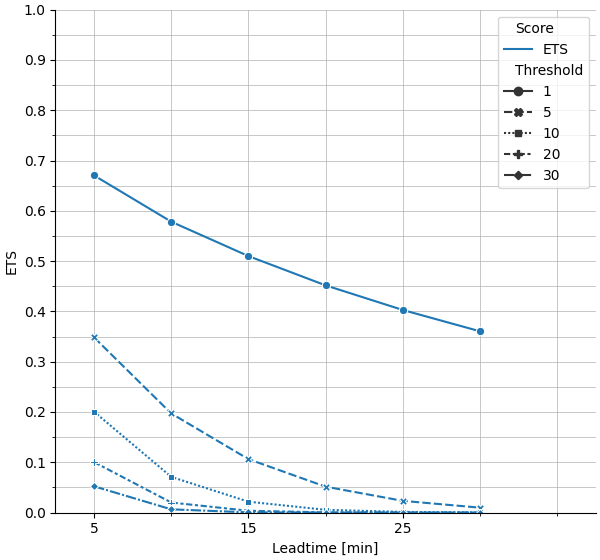
\includegraphics[width=0.33\linewidth]{images/model_choice/sigma_e-2}}
	\subfloat[$\sigma=1e^{-3}$]{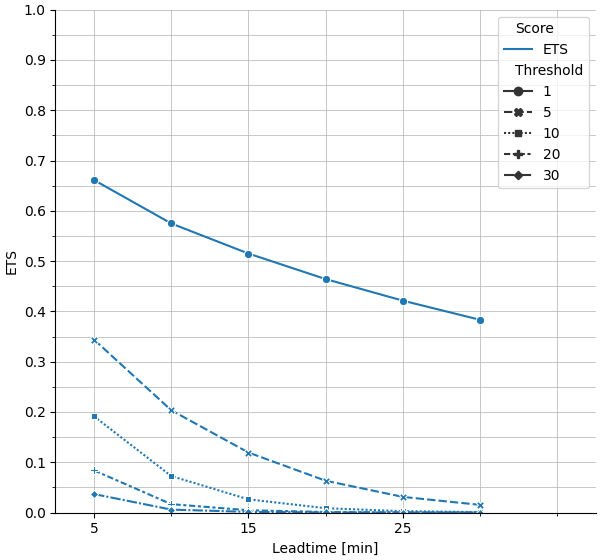
\includegraphics[width=0.33\linewidth]{images/model_choice/sigma_e-3}}
	\subfloat[$\sigma=1e^{-4}$]{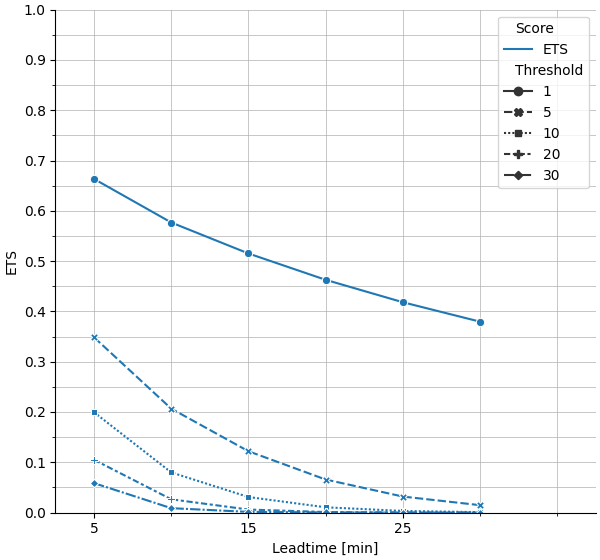
\includegraphics[width=0.33\linewidth]{images/model_choice/sigma_e-4}}
	\caption{ETS scores of RainNet over the validation set at model convergence used for choosing a $\sigma$ Gaussian NLL parameter. Thresholds are expressed in mm/h.}
	\label{fig:sigma_selection}
\end{figure}


\begin{figure}[H]
	\centering
	\subfloat[Equal]{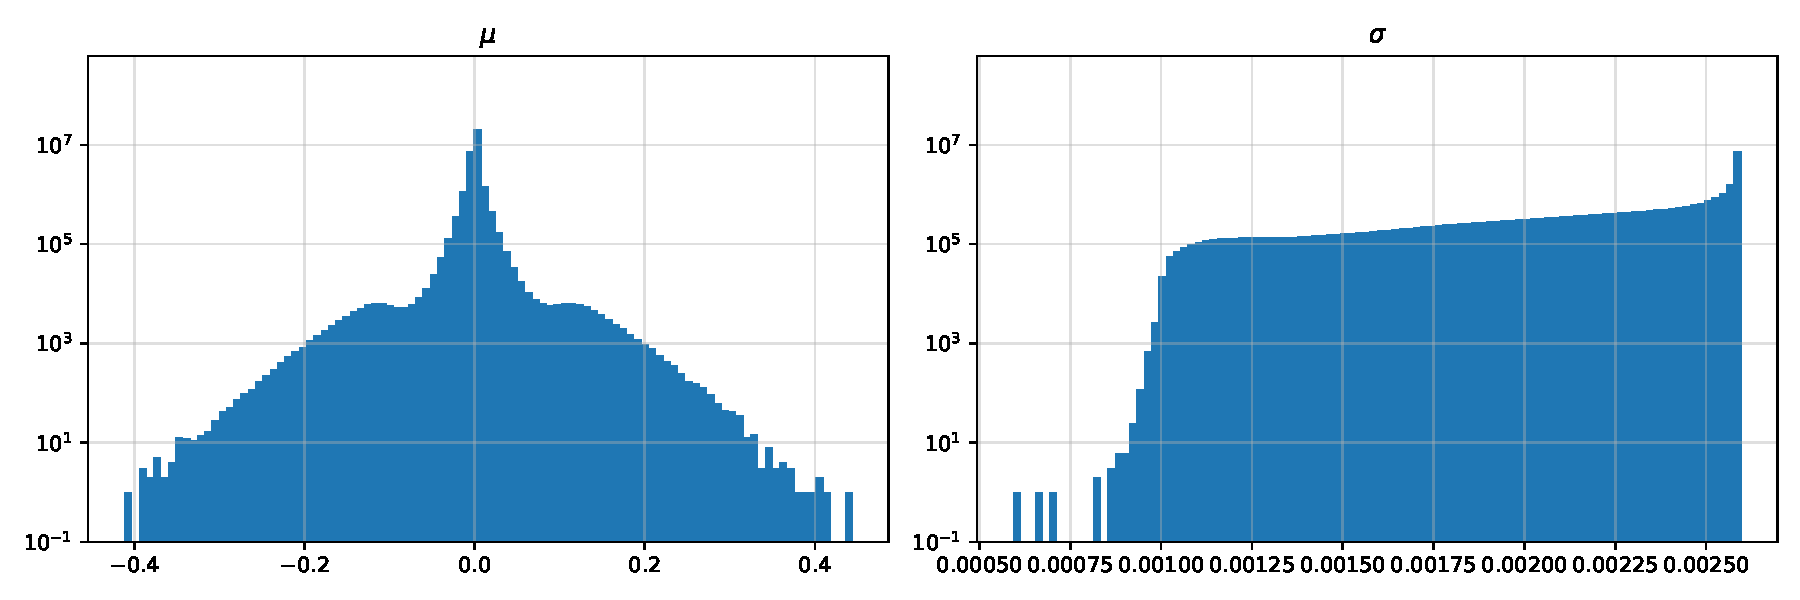
\includegraphics[width=0.5\linewidth]{images/weight/bcnn_t2_gsm_small_diff_lt5}}
	\subfloat[Blundell]{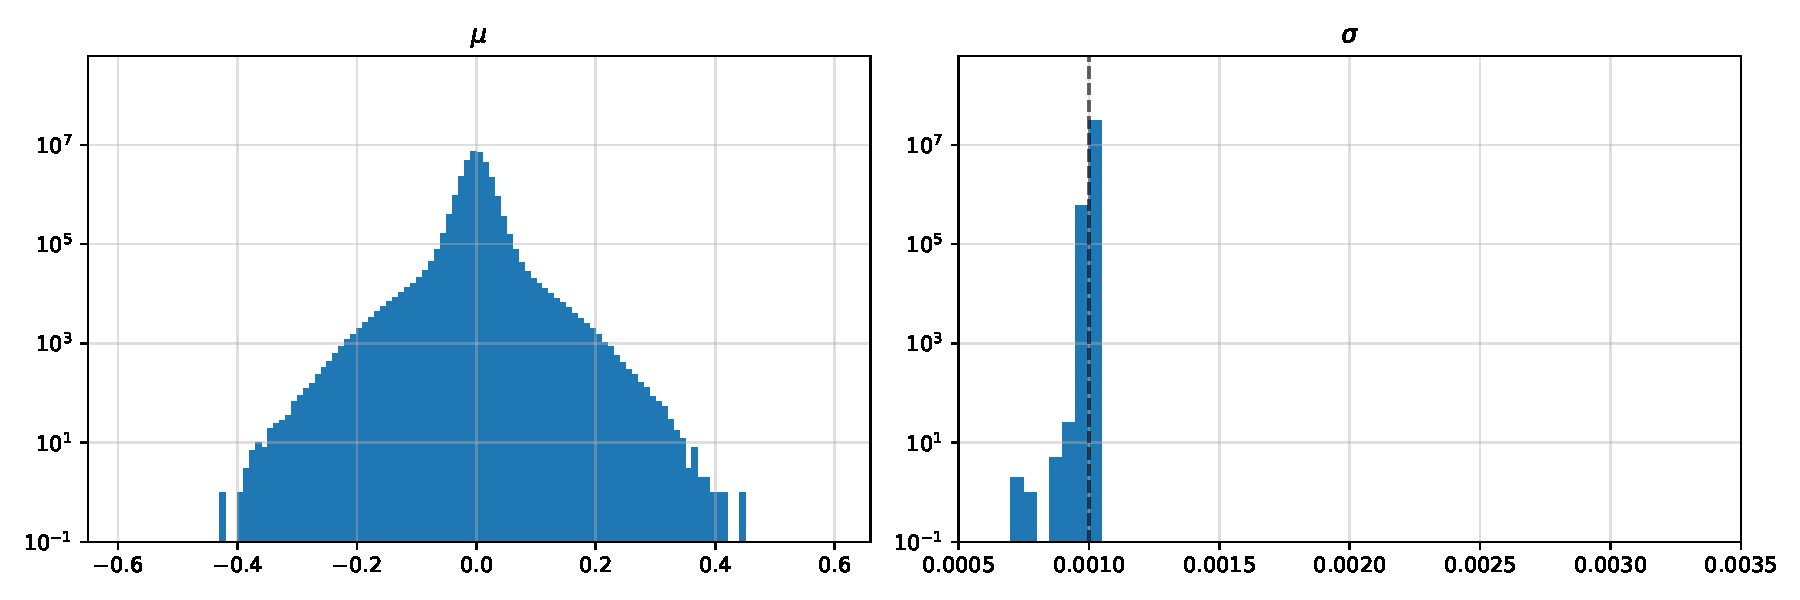
\includegraphics[width=0.5\linewidth]{images/weight/bcnn_t2_gsm_small_diff_blundell_lt5}}
	\subfloat[Epoch]{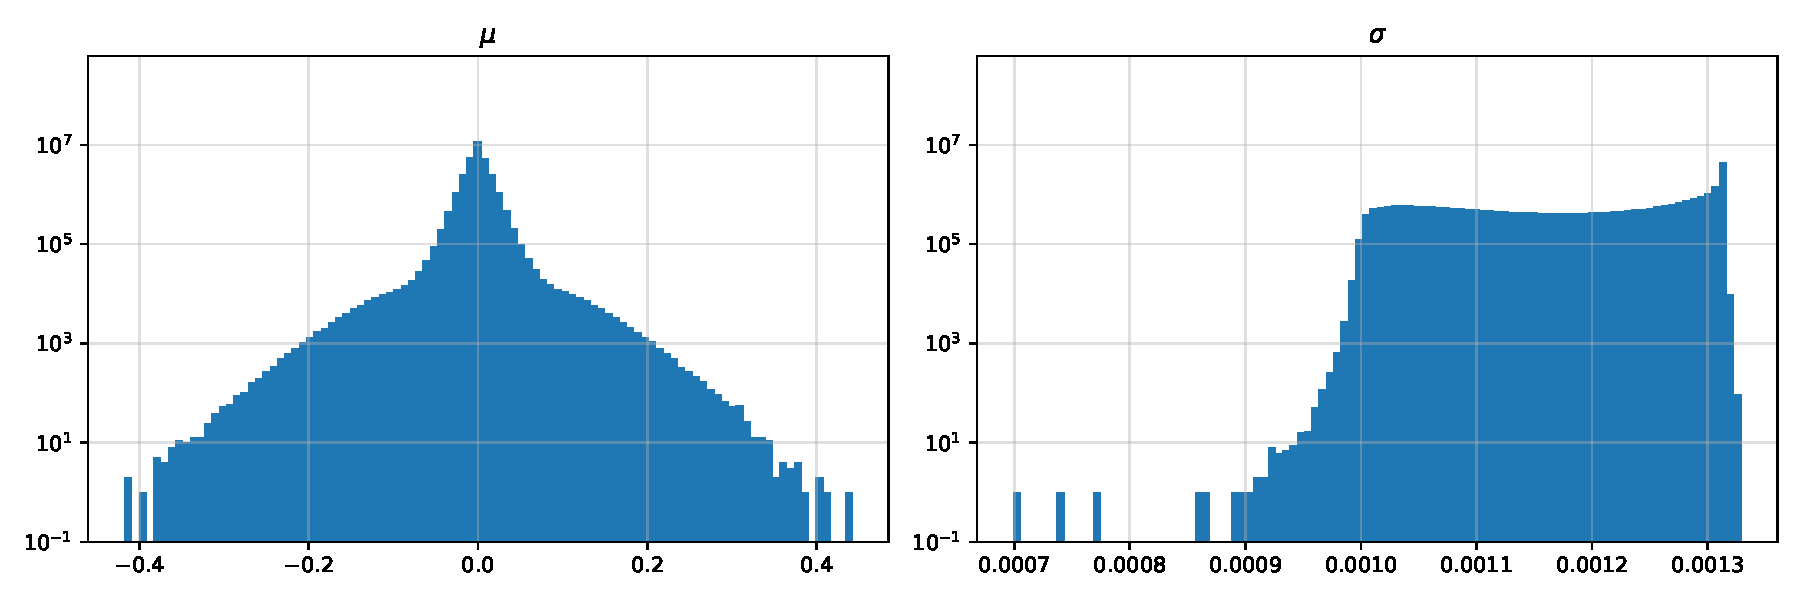
\includegraphics[width=0.5\linewidth]{images/weight/bcnn_t2_gsm_small_diff_epoch_lt5}}
	\caption{The relation of KL-weighting scheme to the parameter posterior distributions across the network. $\mu$ histograms describe the parameter mean distributions, whereas $\sigma$ distributions describe the distribution of their standard deviations. The prior chosen is GSM SD.}
	\label{fig:bcnn-training-weights}
\end{figure}

\pagebreak

\section{Case Studies}
\label{section:additional-case-studies}

\begin{figure}[H]
	\centering
	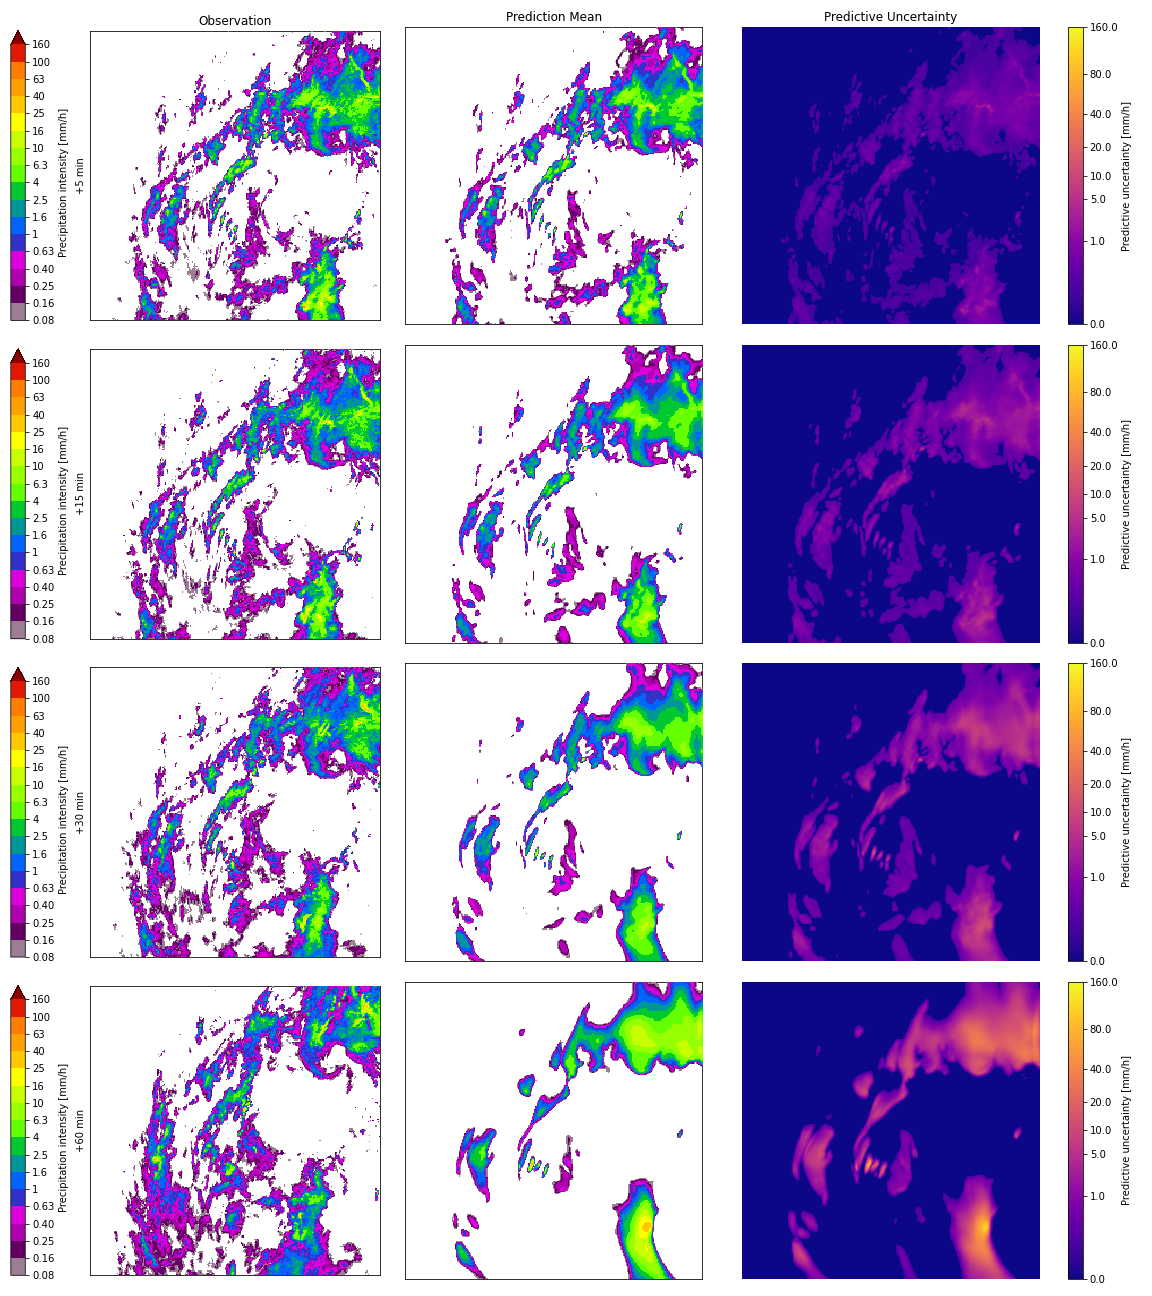
\includegraphics[width=\textwidth]{images/cases/bcnn_better_mean}
	\caption{Predictive mean and uncertainty (two standard deviations) for Case 1 on the 25th of May 2019 starting at 1PM for the \texttt{BCNN lt5 new} model.}
	\label{fig:bcnn_better_mean}
\end{figure}

\begin{figure}[H]
	\centering
	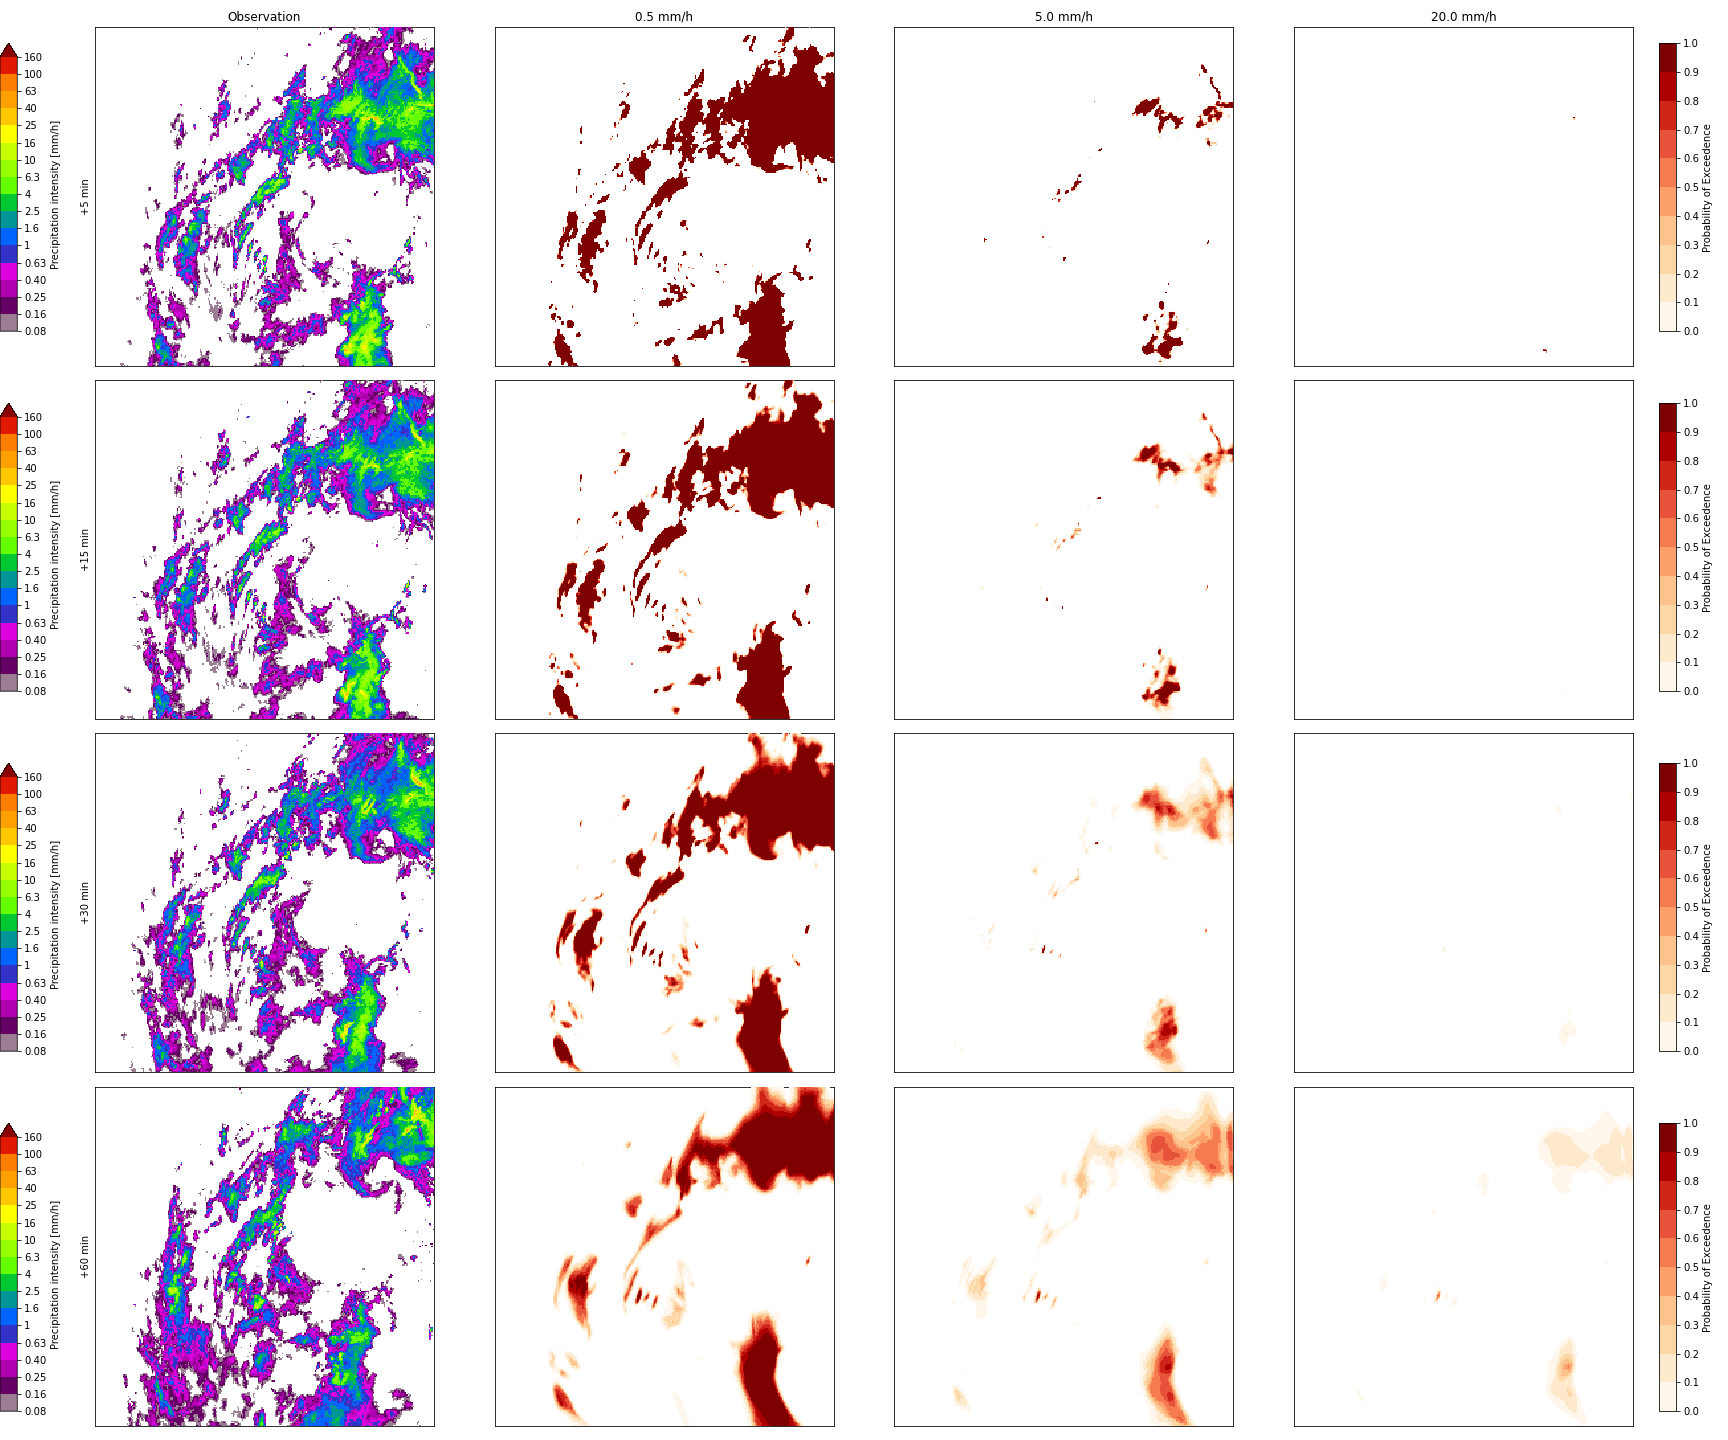
\includegraphics[width=\textwidth]{images/cases/bcnn_better_prob}
	\caption{0.5, 5.0, and 20.0 mm/h exceedance probabilities for Case 1 on the 25th of May 2019 starting at 1PM for the \texttt{BCNN lt5 new} model.}
	\label{fig:bcnn_better_prob}
\end{figure}

\begin{figure}[H]
	\centering
	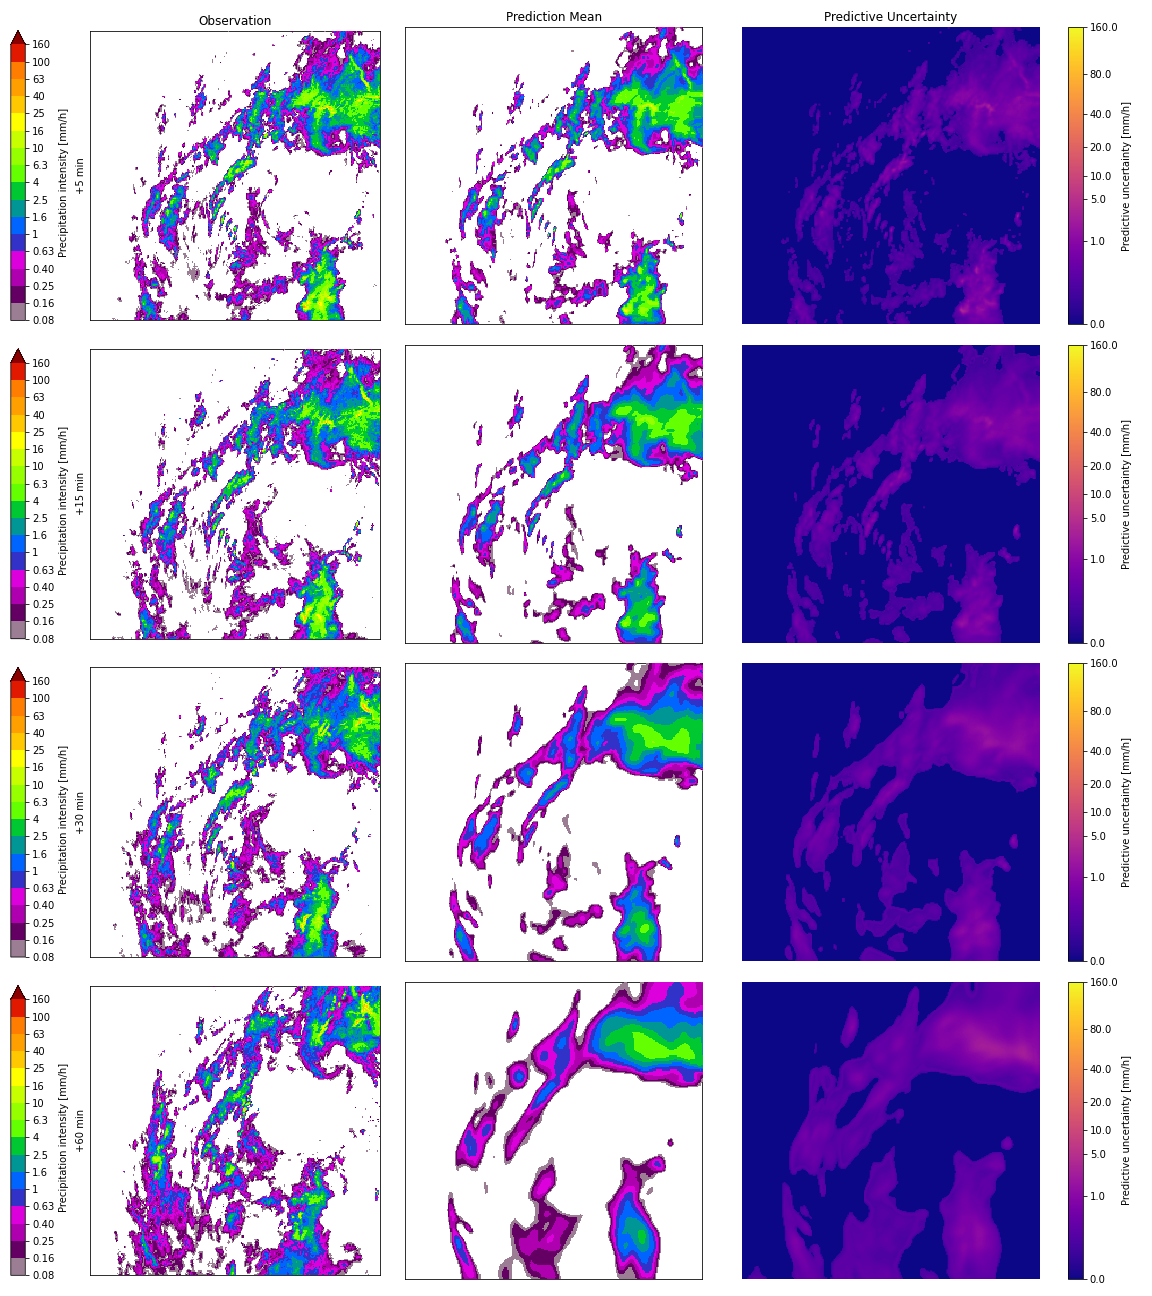
\includegraphics[width=\textwidth]{images/cases/bcnn_p2_lt30_mean}
	\caption{Predictive mean and uncertainty (two standard deviations) for Case 1 on the 25th of May 2019 starting at 1PM for the \texttt{BCNN lt30} model.}
	\label{fig:bcnn_p2_lt30_mean}
\end{figure}

\begin{figure}[H]
	\centering
	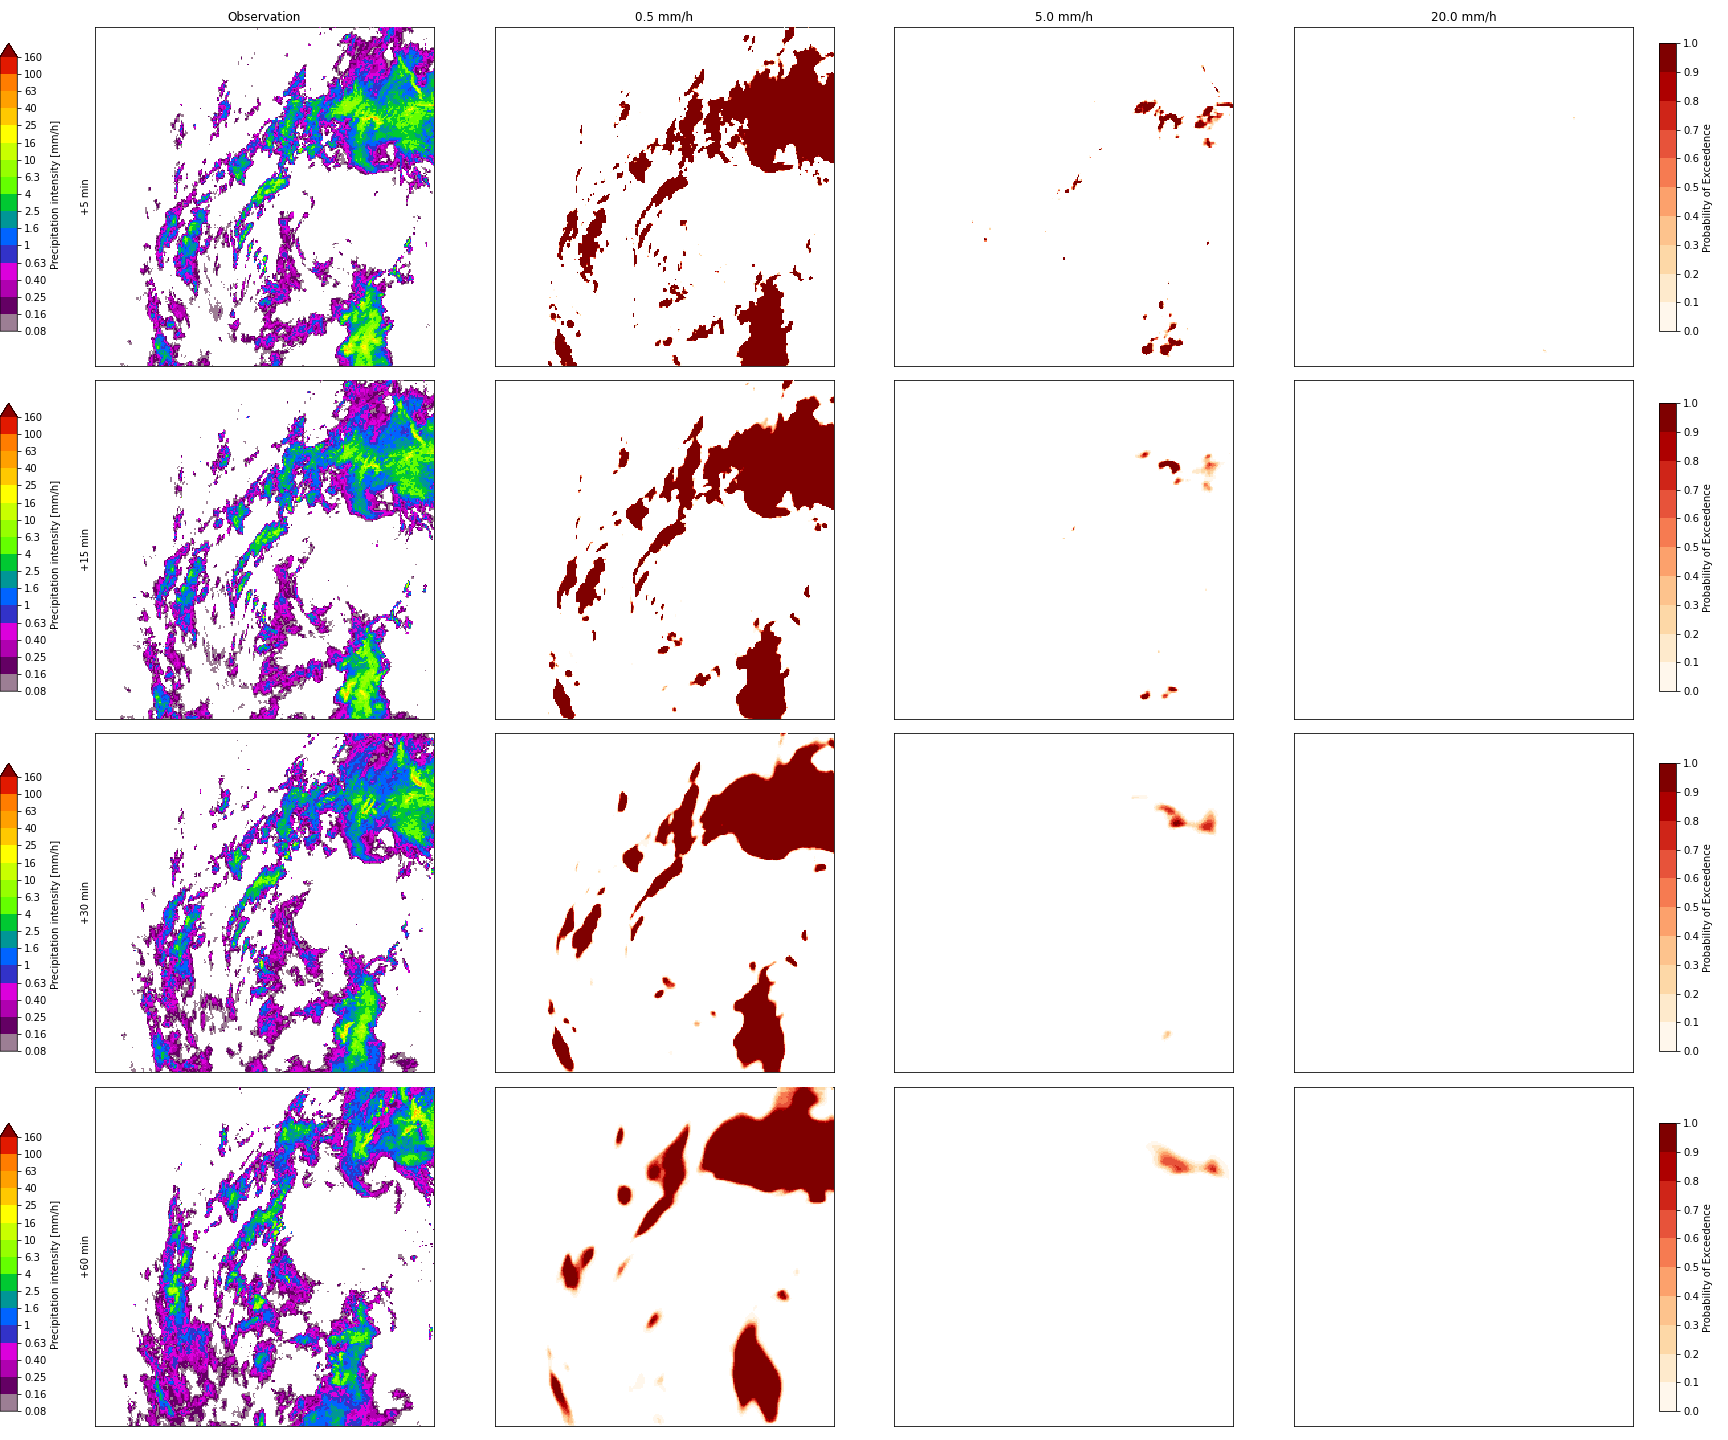
\includegraphics[width=\textwidth]{images/cases/bcnn_p2_lt30_prob}
	\caption{0.5, 5.0, and 20.0 mm/h exceedance probabilities for Case 1 on the 25th of May 2019 starting at 1PM for the \texttt{BCNN lt30} model.}
	\label{fig:bcnn_p2_lt30_prob}
\end{figure}

\begin{figure}[H]
	\centering
	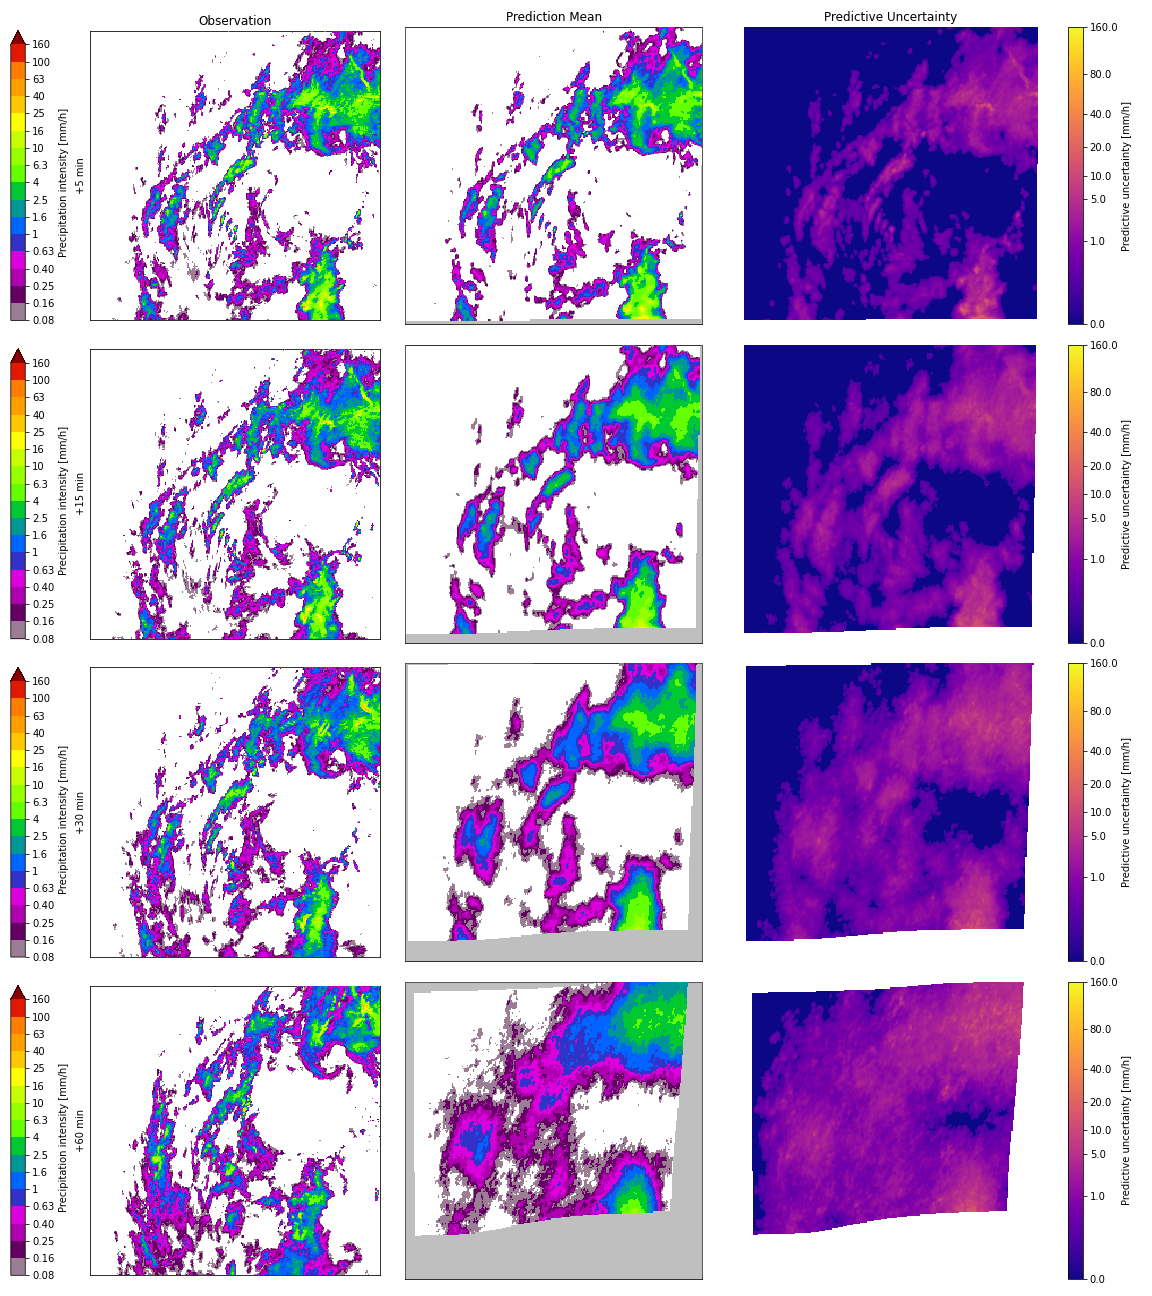
\includegraphics[width=\textwidth]{images/cases/steps_mean}
	\caption{Predictive mean and uncertainty (two standard deviations) for Case 1 on the 25th of May 2019 starting at 1PM for the baseline STEPS model.}
	\label{fig:steps_mean}
\end{figure}

\begin{figure}[H]
	\centering
	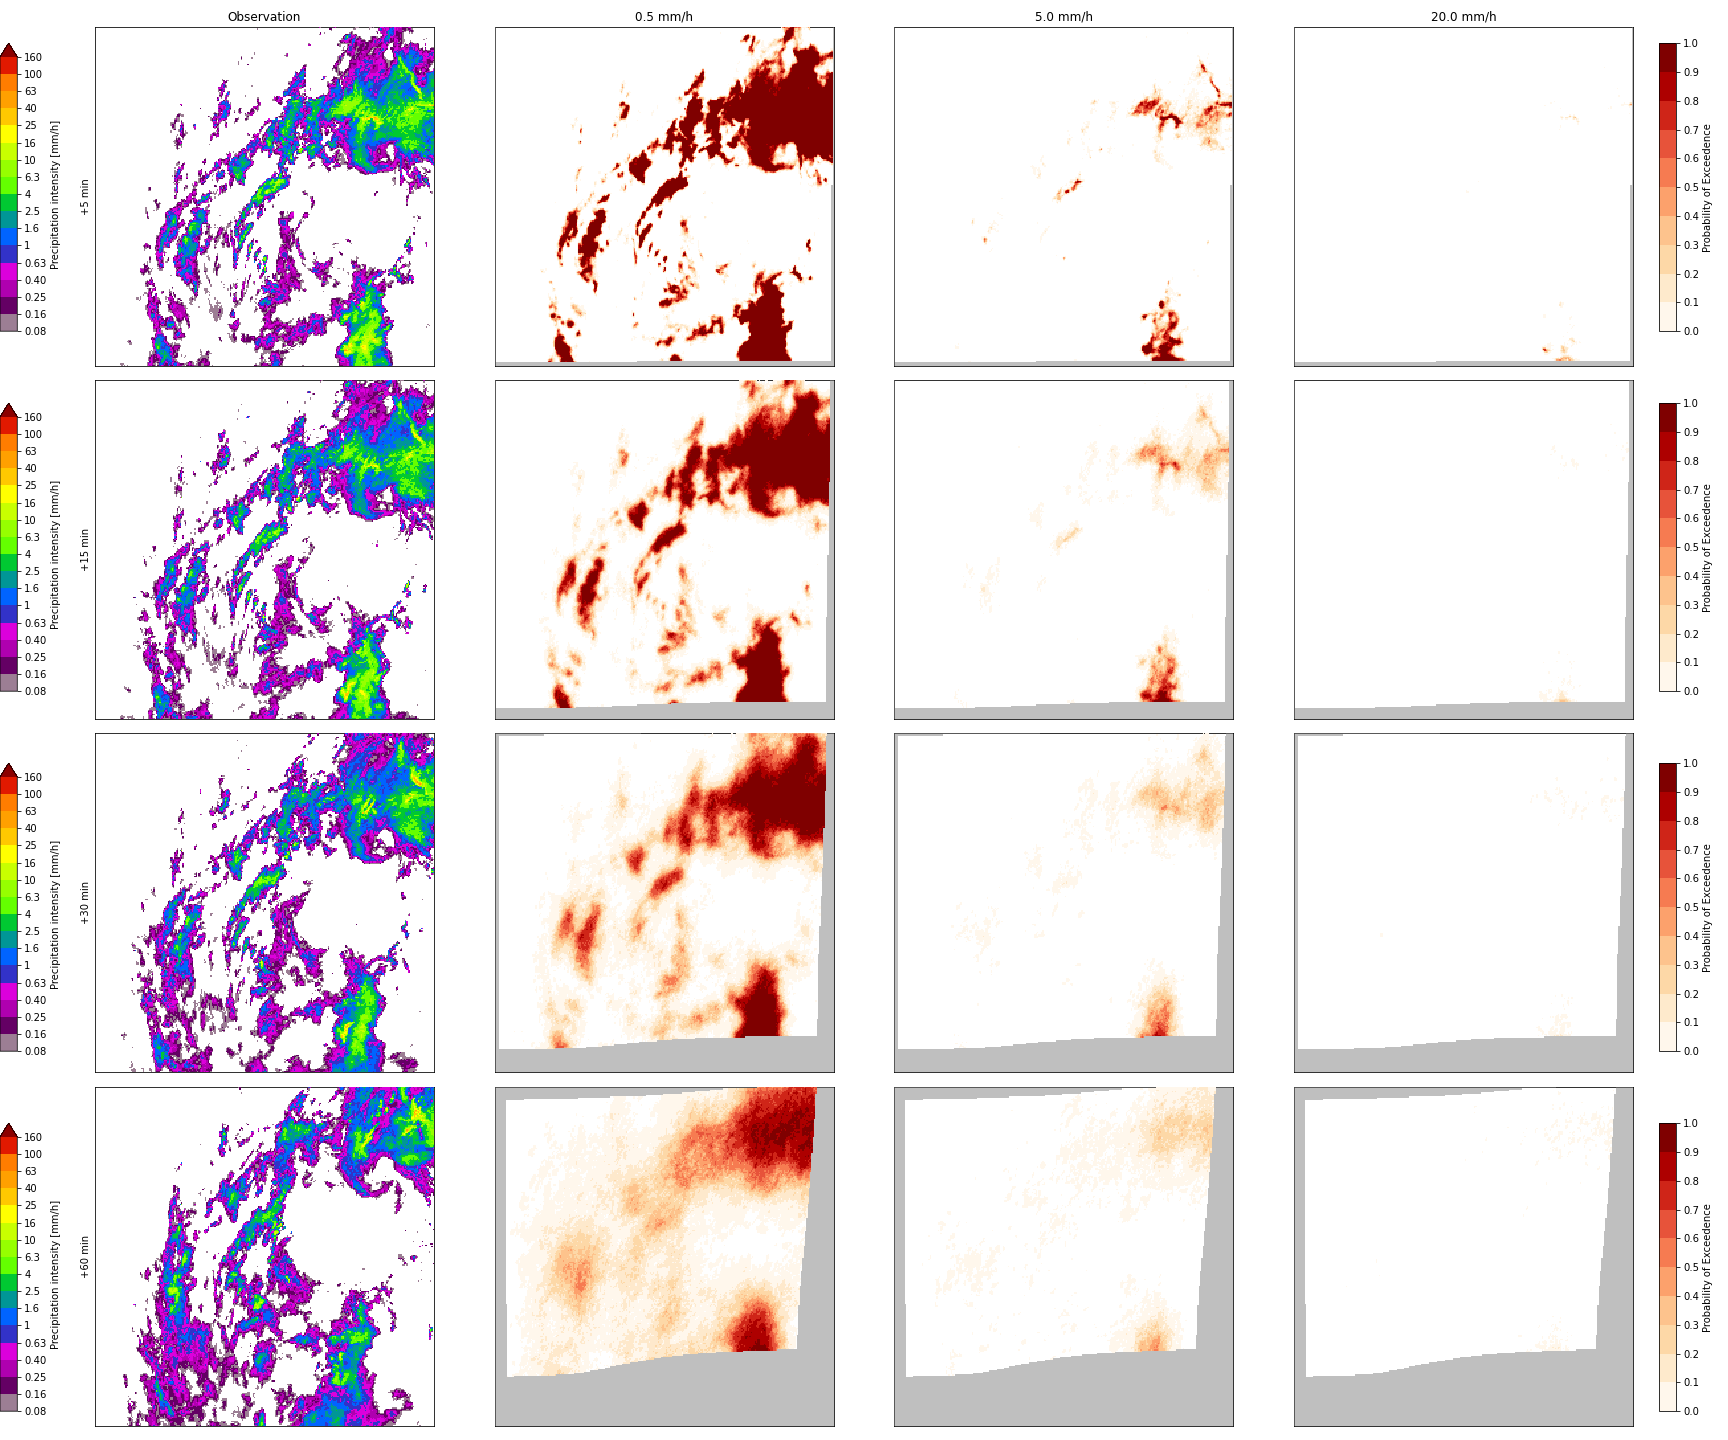
\includegraphics[width=\textwidth]{images/cases/steps_prob}
	\caption{0.5, 5.0, and 20.0 mm/h exceedance probabilities for Case 1 on the 25th of May 2019 starting at 1PM for the baseline STEPS model.}
	\label{fig:steps_prob}
\end{figure}

\section{Deterministic Metrics}

\begin{figure}[H]
	\subfloat[0.5 mm/h]{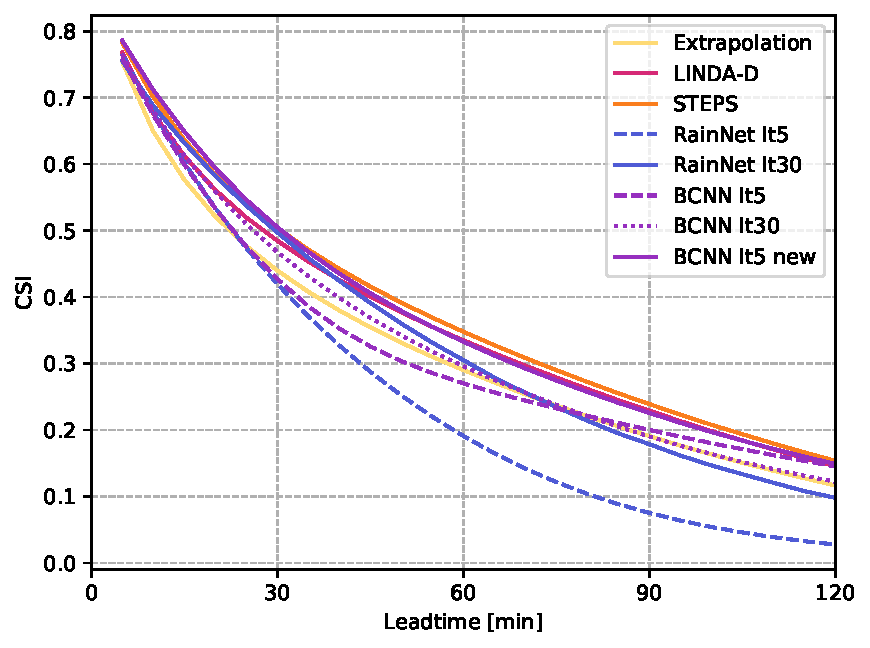
\includegraphics[width=0.33\textwidth]{images/metrics/ALL_CSI_0_5}}%
	\subfloat[5.0 mm/h]{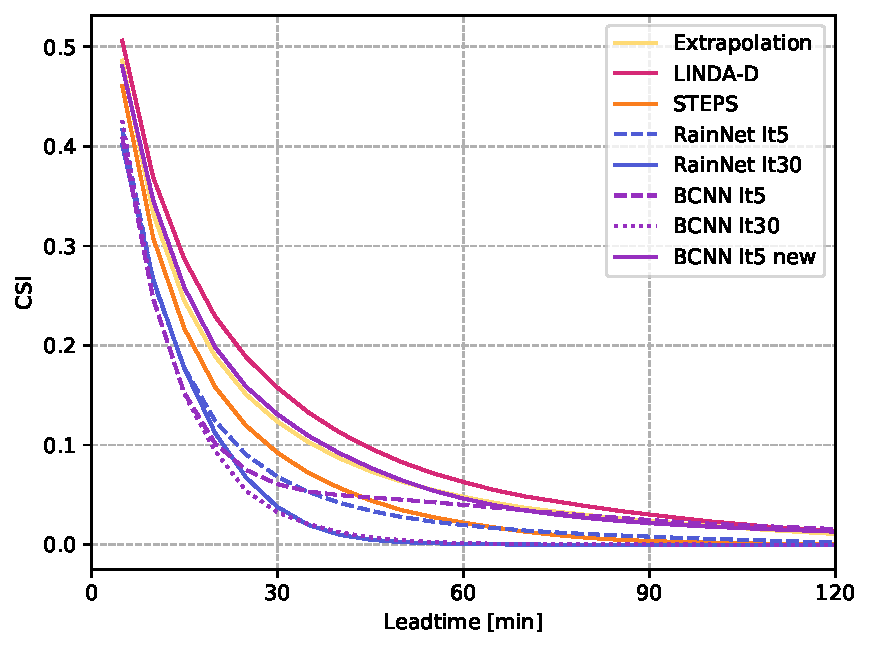
\includegraphics[width=0.33\textwidth]{images/metrics/ALL_CSI_5_0}}%
	\subfloat[20.0 mm/h]{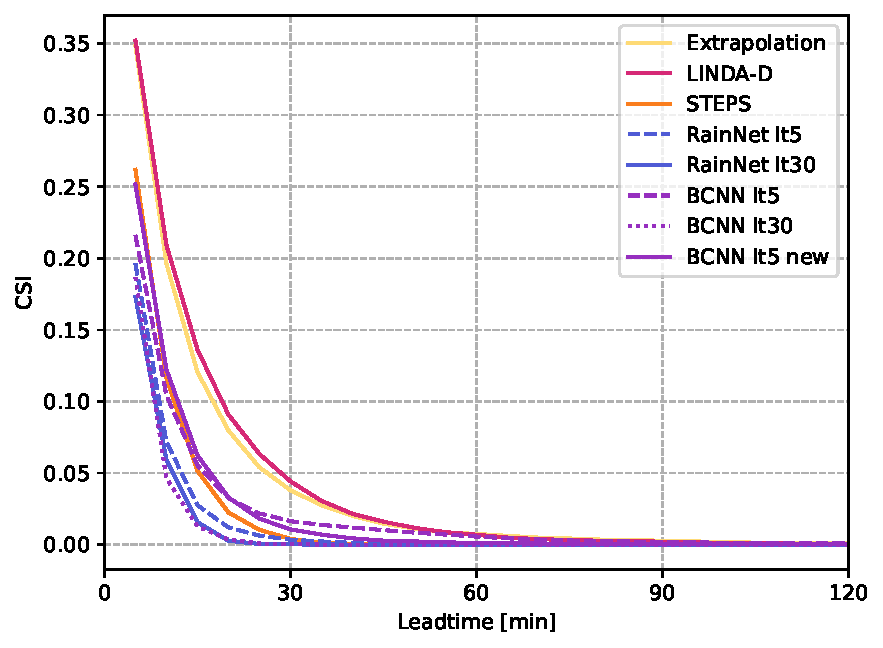
\includegraphics[width=0.33\textwidth]{images/metrics/ALL_CSI_20_0}}%
	\caption{CSI scores}
	\label{fig:csi}
\end{figure}

\begin{figure}[H]
	\subfloat[0.5 mm/h]{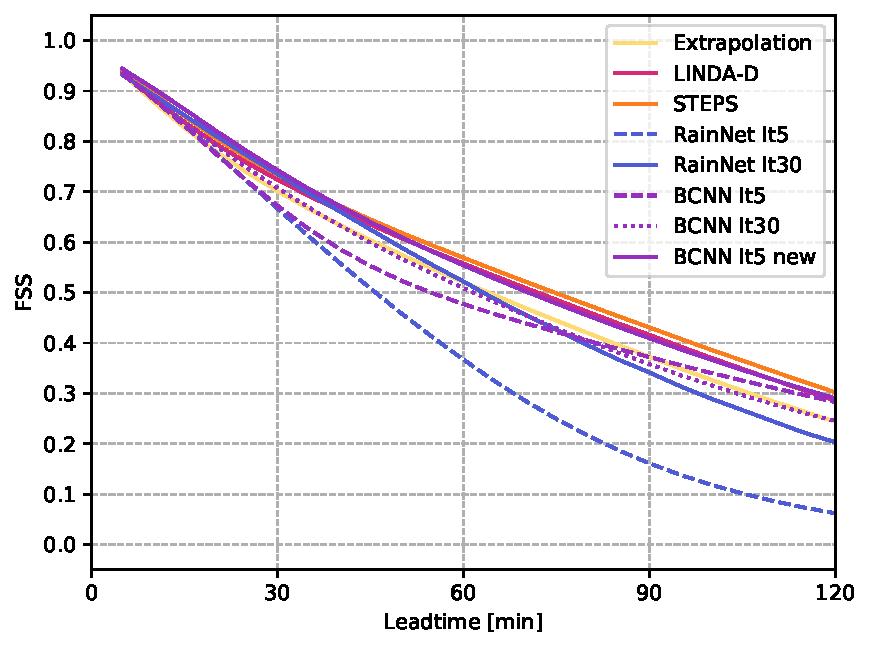
\includegraphics[width=0.33\textwidth]{images/metrics/ALL_FSS_2_0_5}}%
	\subfloat[5.0 mm/h]{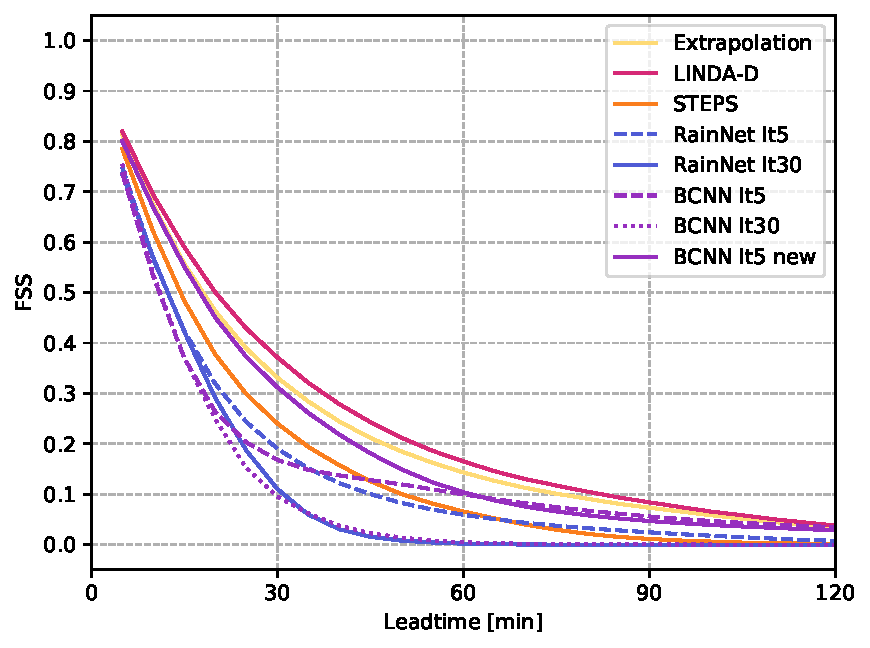
\includegraphics[width=0.33\textwidth]{images/metrics/ALL_FSS_2_5_0}}%
	\subfloat[20.0 mm/h]{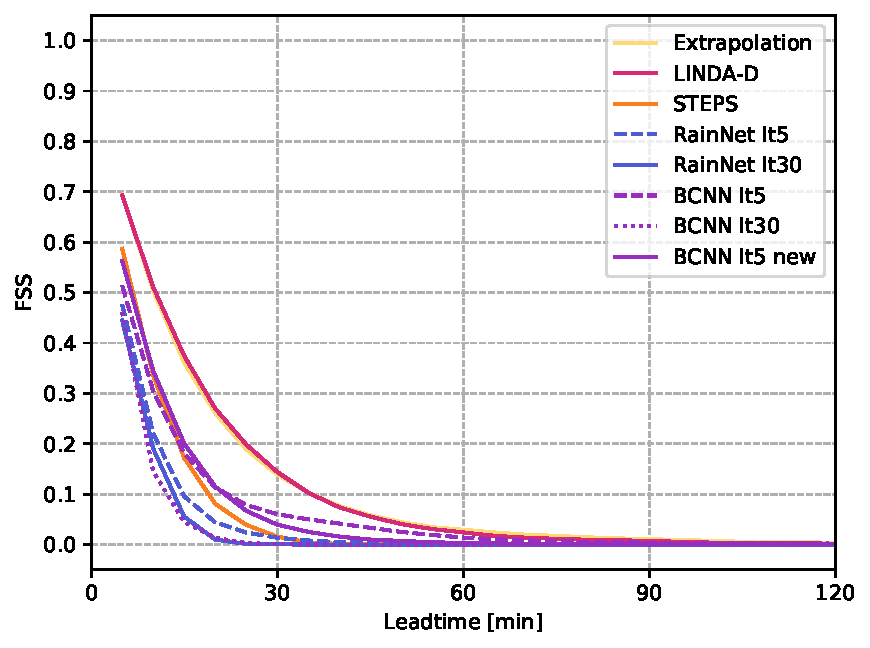
\includegraphics[width=0.33\textwidth]{images/metrics/ALL_FSS_2_20_0}}%
	\caption{FSS scores (4km)}
	\label{fig:fss4}
\end{figure}

\section{Probabilistic Metrics}


\begin{figure}[H]
	\centering
	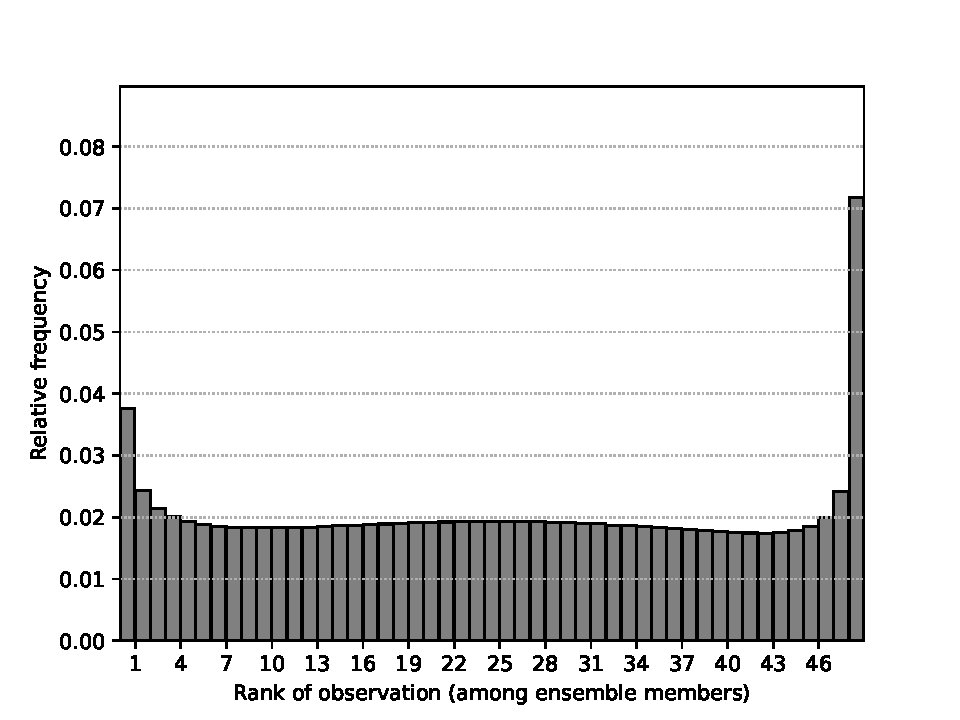
\includegraphics[width=\textwidth]{images/metrics/linda-p_rankhist_l_12}
	\caption{Rank Histogram for LINDA-P model nowcasts at a one-hour leadtime, for precipitation events exceeding 0.1 mm/h}
	\label{fig:rankhist_linda}
\end{figure}



% End of document!
% ------------------------------------------------------------------
% The LastPage package automatically places a label on the last page.
% That works better than placing a label here manually, because the
% label might not go to the actual last page, if LaTeX needs to place
% floats (that is, figures, tables, and such) to the end of the 
% document.
\end{document}
